\documentclass[10pt]{beamer}%
\usetheme[progressbar = foot]{metropolis} 
\usecolortheme[cautious]{owl} %owl-defined colours will be available as OwlRed, OwlGreen, and so forth.
\setbeamercolor{title separator}{fg=OwlGreen}

% input

\usepackage[utf8]{inputenc}%
\usepackage{lmodern} %Type1-font for non-english texts and characters
\usepackage[USenglish]{babel} %francais, polish, spanish, ...
\usepackage[T1]{fontenc}

\usepackage{ragged2e}%for text justification by default
\justifying

% graphics
%% Figures %%%%%%%%%%%%%%%%%%%%%%%%%%%%%%%%%%%%%%%%%%%%%%%%%%
\usepackage{graphicx}
\usepackage{xcolor}%for color mixing
\definecolor{mypurple}{rgb}{0.231, 0.204, 0.471}
\definecolor{mypurple1}{rgb}{0.573, 0.467, 0.675}
\definecolor{mypurple2}{rgb}{0.122, 0.016, 0.224}

\definecolor{mygreen}{rgb}{0.153, 0.443, 0.365}
\definecolor{myorange}{rgb}{0.882, 0.612, 0.224}

\definecolor{bostonuniversityred}{rgb}{0.8, 0.0, 0.0}
\definecolor{blendedblue}{rgb}{0.137,0.466,0.741}

\definecolor{darkred}{rgb}{0.545,0,0}

 
\usepackage{tikz} % for arrows and figures
\usetikzlibrary{positioning,decorations.pathreplacing,shapes,trees,calc}

\makeatletter
\newcommand{\gettikzxy}[3]{%
  \tikz@scan@one@point\pgfutil@firstofone#1\relax
  \edef#2{\the\pgf@x}%
  \edef#3{\the\pgf@y}%
}

\usepackage{amsmath}%
\usepackage{amsfonts}%
\usepackage{amssymb}%
\usepackage{graphicx}


\usepackage{booktabs}


\usepackage{hyperref}
\setlength{\arraycolsep}{3pt}

%%%%%%%%%%%%%%%%%%%%%%%%%%%%%%%%%%%%%%%%%%%%%%
%%%%%%%%%%%%%%%%% Doc info %%%%%%%%%%%%%%%%%%%
\title[\textbf{Adaptation against apparent selection}]{\textbf{Individual-level causes and population-level consequences of variation in fitness in an Alpine rodent}}
%\titlegraphic{\fcolorbox{blendedblue}{blendedblue}{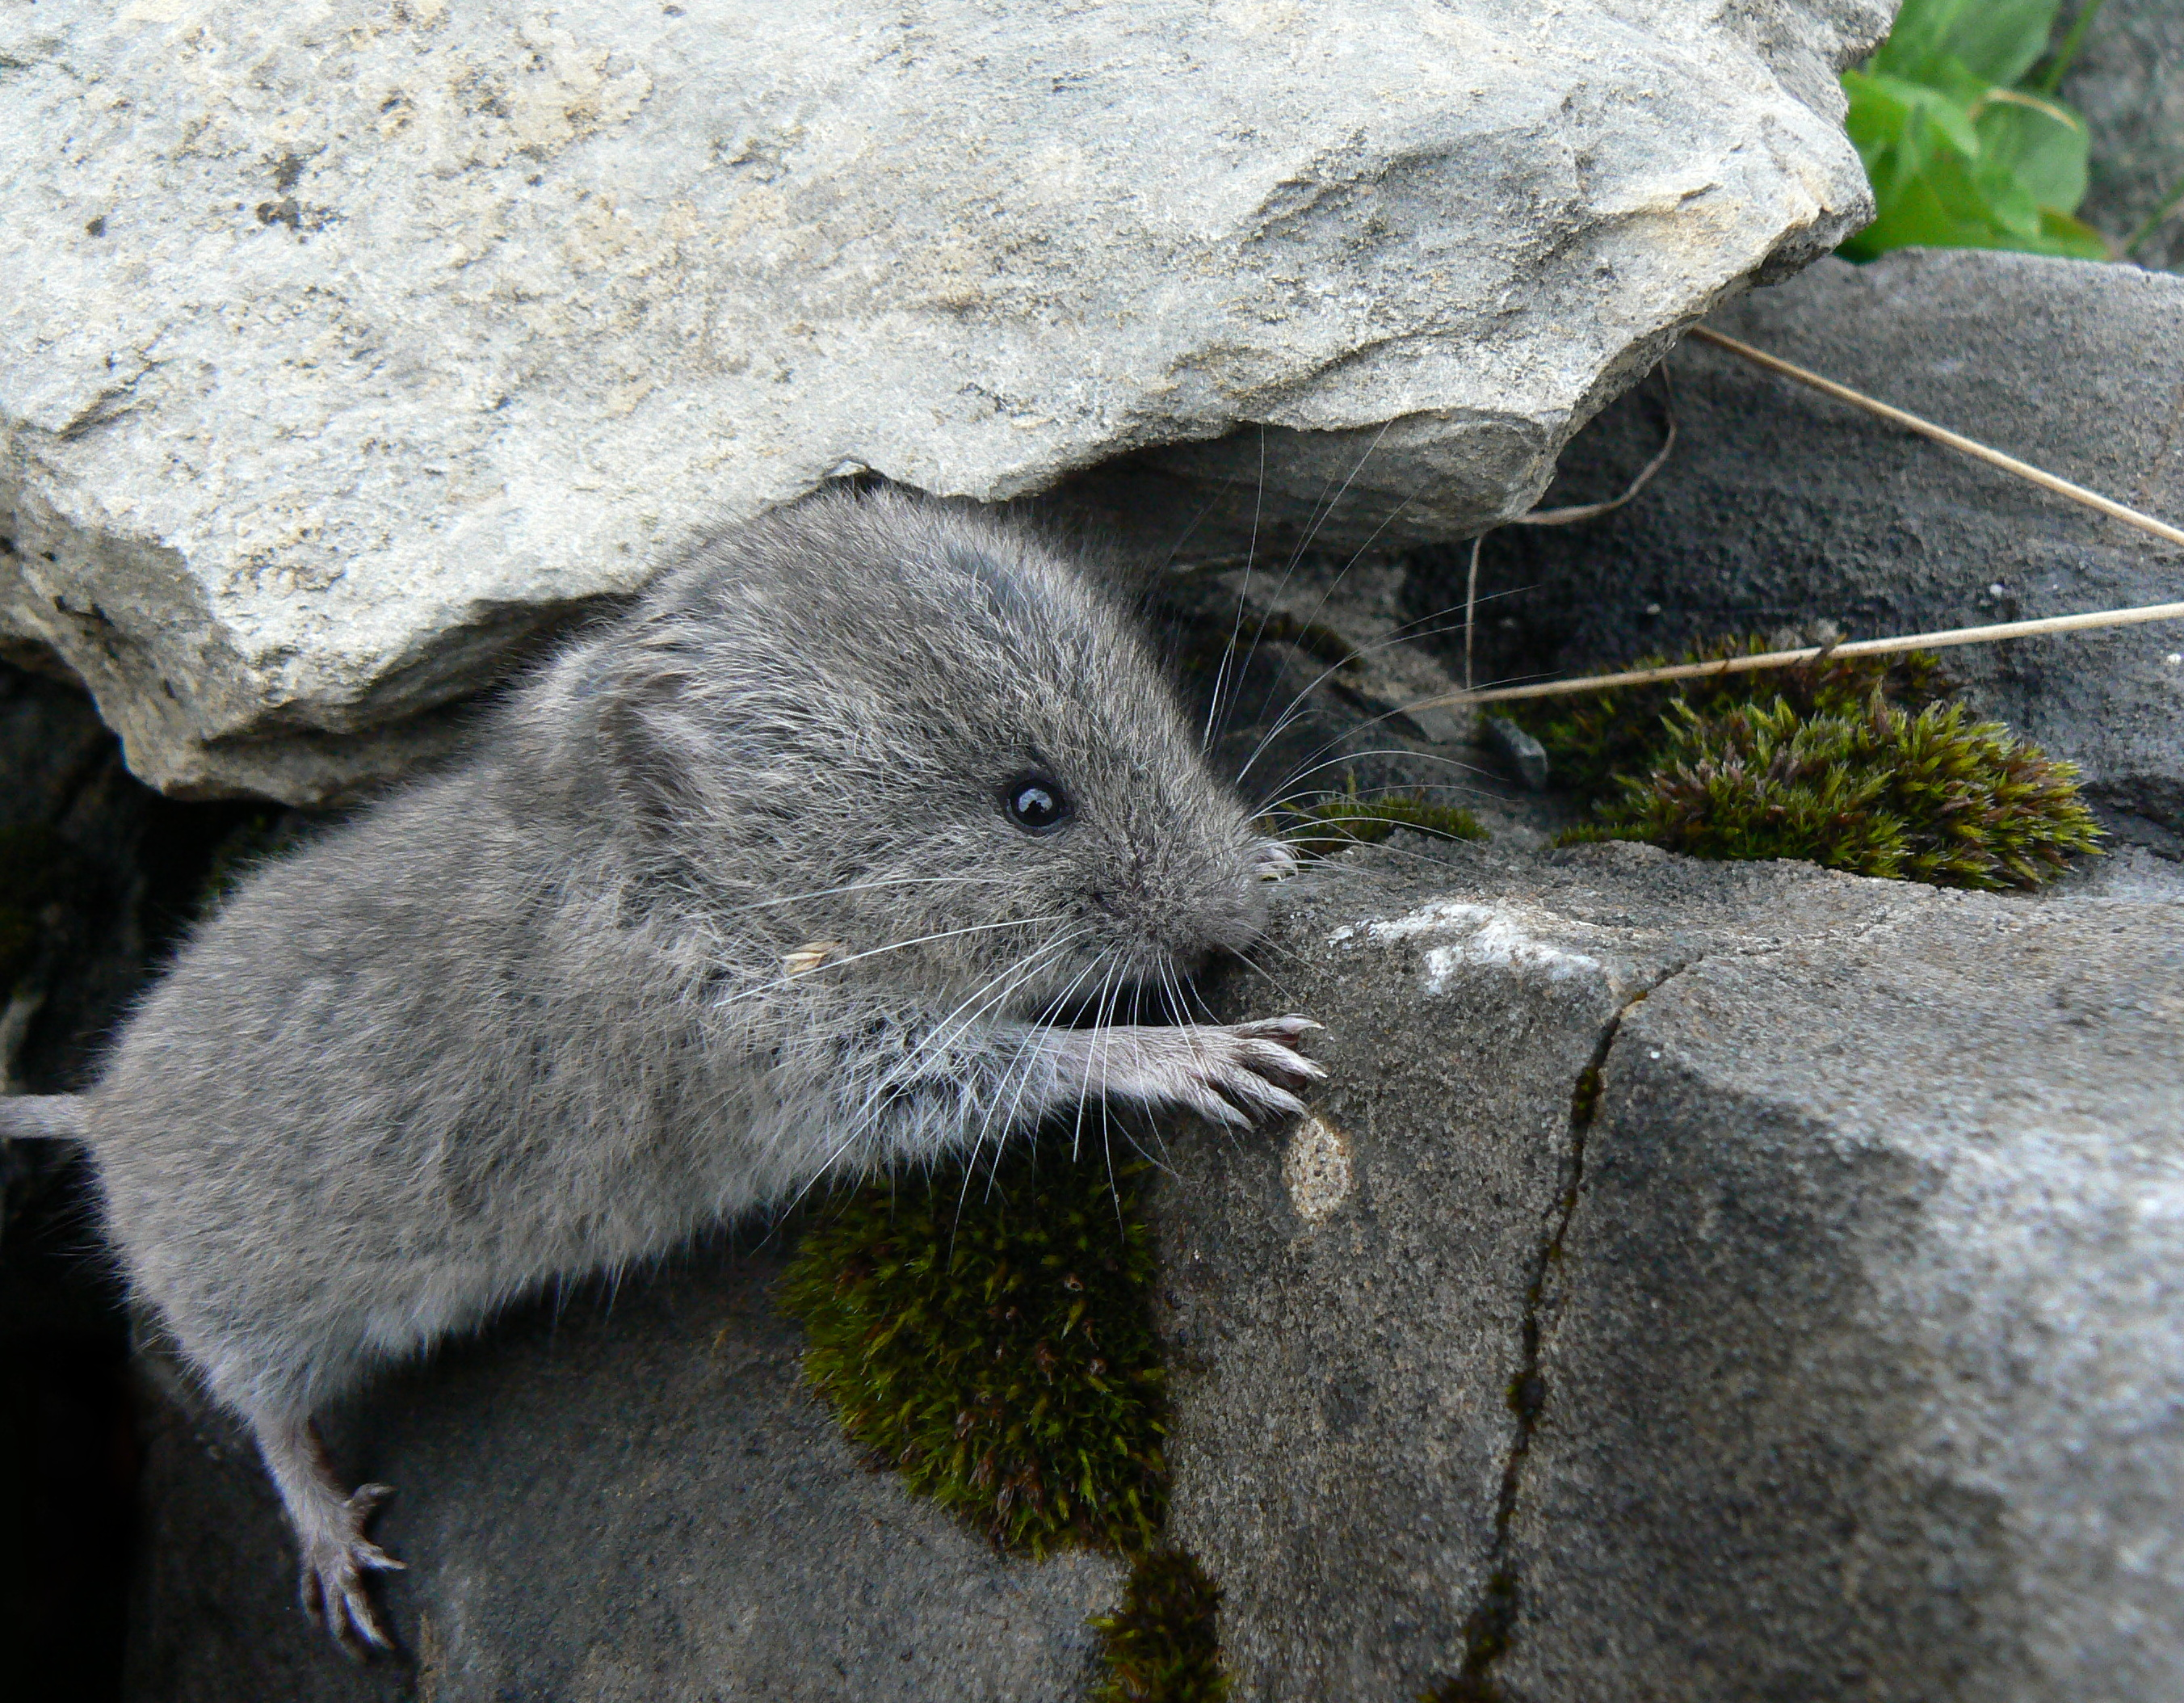
\includegraphics[width=0.45\textwidth]{Figures/cutevole}}}
%\subtitle{UOBU}
\author[\textbf{\fontfamily{pcr}\selectfont timothee.bonnet@ieu.uzh.ch}]{\textbf{Timoth\'{e}e Bonnet}}
%\date{\fcolorbox{blendedblue}{blendedblue}{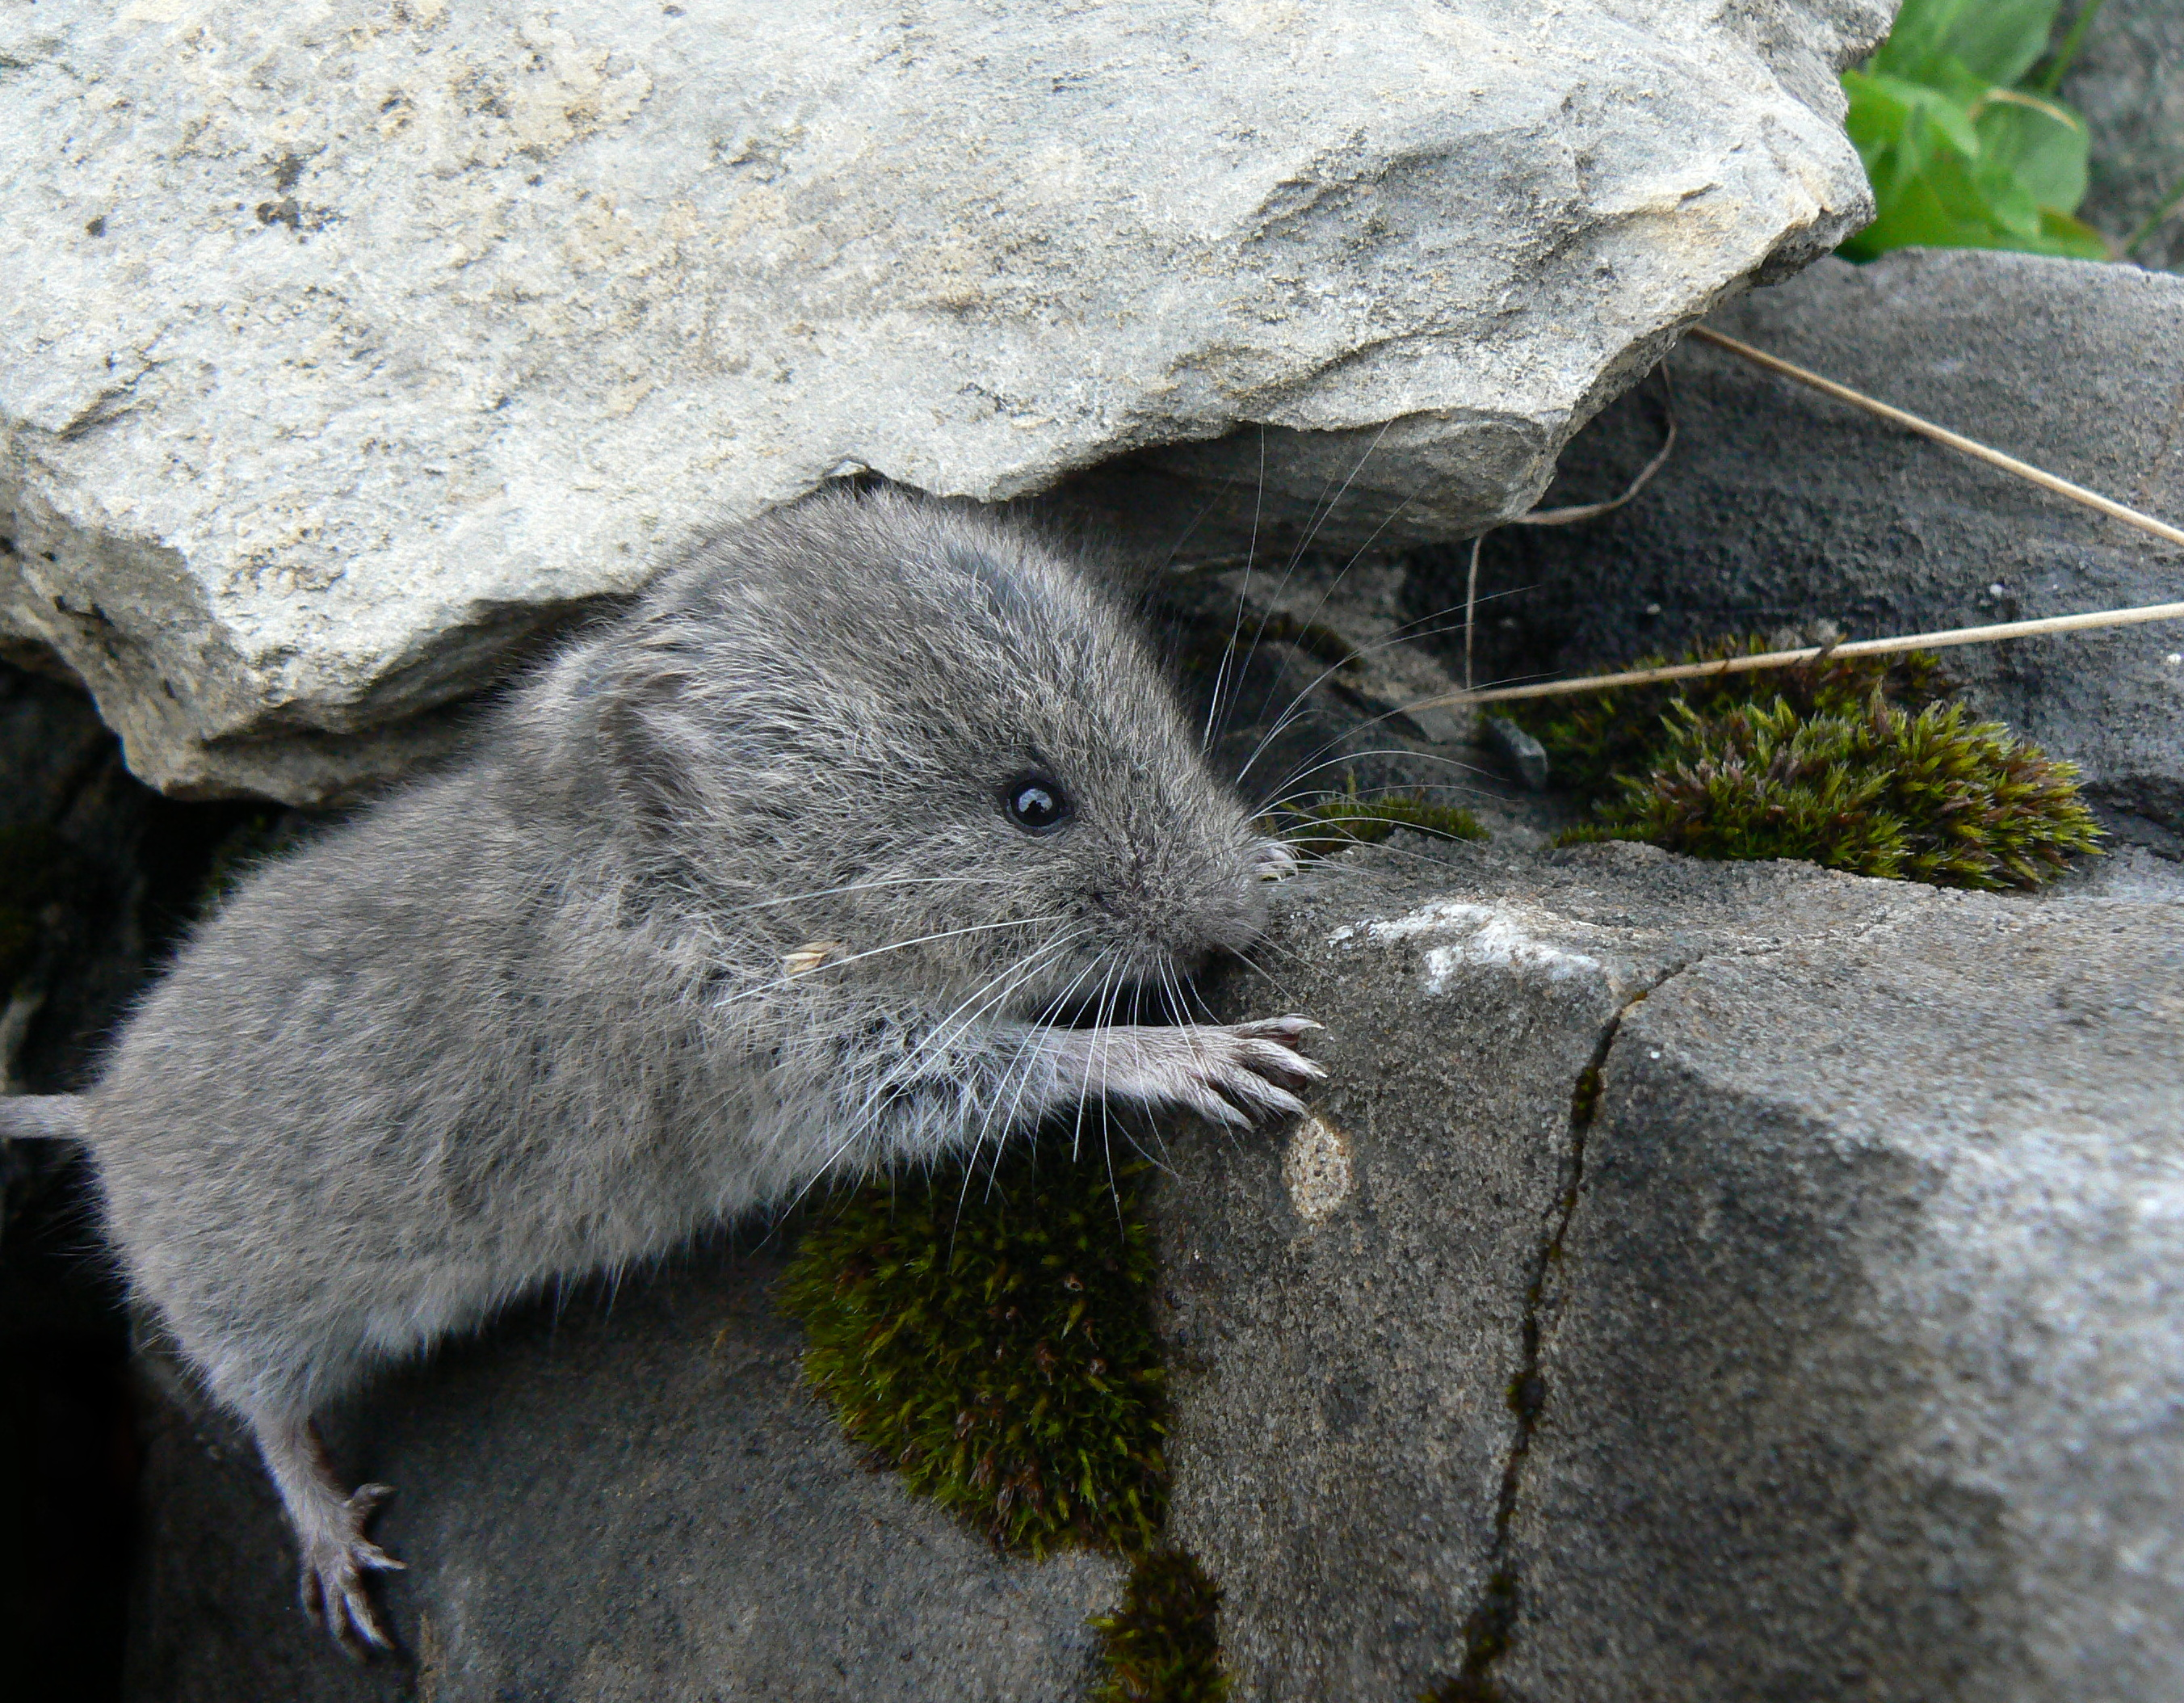
\includegraphics[width=0.35\textwidth]{Figures/cutevole}}}
\date{\vspace{1cm}}
\institute[IEU, University of Zurich]{\small Department of evolutionary biology and environmental studies (IEU) \\ \vspace{-0.1cm} \\ 
\includegraphics[width=0.3\textwidth]{Figures/uzh_logo_e_neg}}



%%%%%%%%%%%%%%%%%%%%%%%%%%%%%%%%%%%%%%%%%%%%%%
\begin{document}

\begin{frame}[plain]
\maketitle
\end{frame}
%%%%%%%%%%%

%\section{Acknowledgements}

\begin{frame}[plain]

\begin{columns}
	\begin{column}[c]{0.35\textwidth}
		\begin{itemize}
		\setlength\itemsep{0.05cm}
		\small
			\item<2-> Erik Postma
		%committee
			\item<3-> Lukas Keller
			\item<3-> Barbara Tschirren
			\item<3-> Arpat Ozgul
			\item<3-> Marc Kéry 
			\item<3-> Jarrod Hadfield
		%colleagues
			\item<4-> Glauco Camenisch
			\item<5-> Ursina Tobler
			\item<6-> Dominique Waldvogel
			\item<6-> Martina Schenkel
			\item<6-> Vicente Garc{\'{i}}a-Navas
			\item<7-> Andres Hagmayer
			\item<8-> Koen van Benthem
			\item<8-> Marjolein Bruijning
			\item<8-> Eelke Jongejans	
			\item<9-> Pirmin Nietlisbach
			\item<9-> Philipp Becker
			\item<9-> Judith Bachmann
					
%former colleagues?

%friends and family
		\end{itemize}
	\end{column}
	\begin{column}[c]{0.7\textwidth}
		%Residual
		\begin{figure}[c]
			\begin{tikzpicture}
				\uncover<2->{\node (erik) at (0,0) {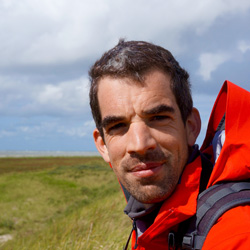
\includegraphics[width = 0.2 \textwidth]{Figures/Erik}};}
				\uncover<3->{\node (lukas) at ($(erik)+(1.2,0)$) {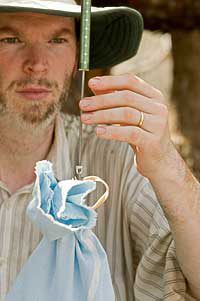
\includegraphics[width = 0.15 \textwidth]{Figures/Lukas}};
				\node (barbara) at ($(lukas)+(1,0)$) {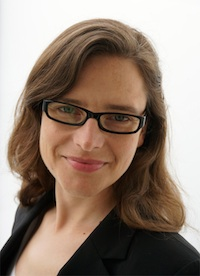
\includegraphics[width = 0.15 \textwidth]{Figures/Barbara}};
				\node (arpat) at ($(barbara)+(1.3,0)$) {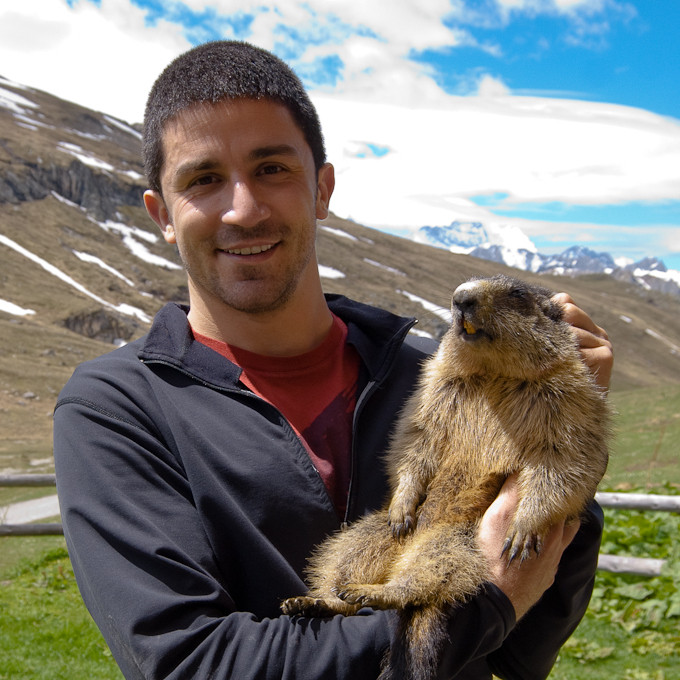
\includegraphics[width = 0.2 \textwidth]{Figures/Arpat}};
				\node (marc) at ($(arpat)+(1.2,0)$) {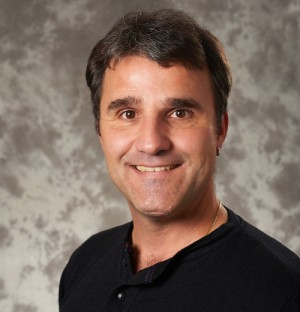
\includegraphics[width = 0.2 \textwidth]{Figures/Marc}};
				\node (jarrod) at ($(marc)+(1.3,0)$) {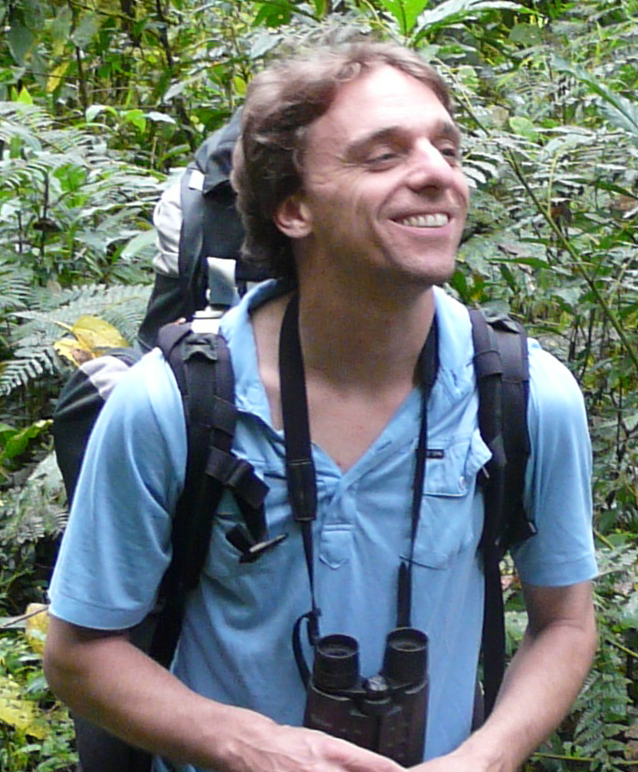
\includegraphics[width = 0.2\textwidth]{Figures/Jarrod}};}
				\uncover<4->{\node (glauco) at ($(erik)+(0,-1.4)$) {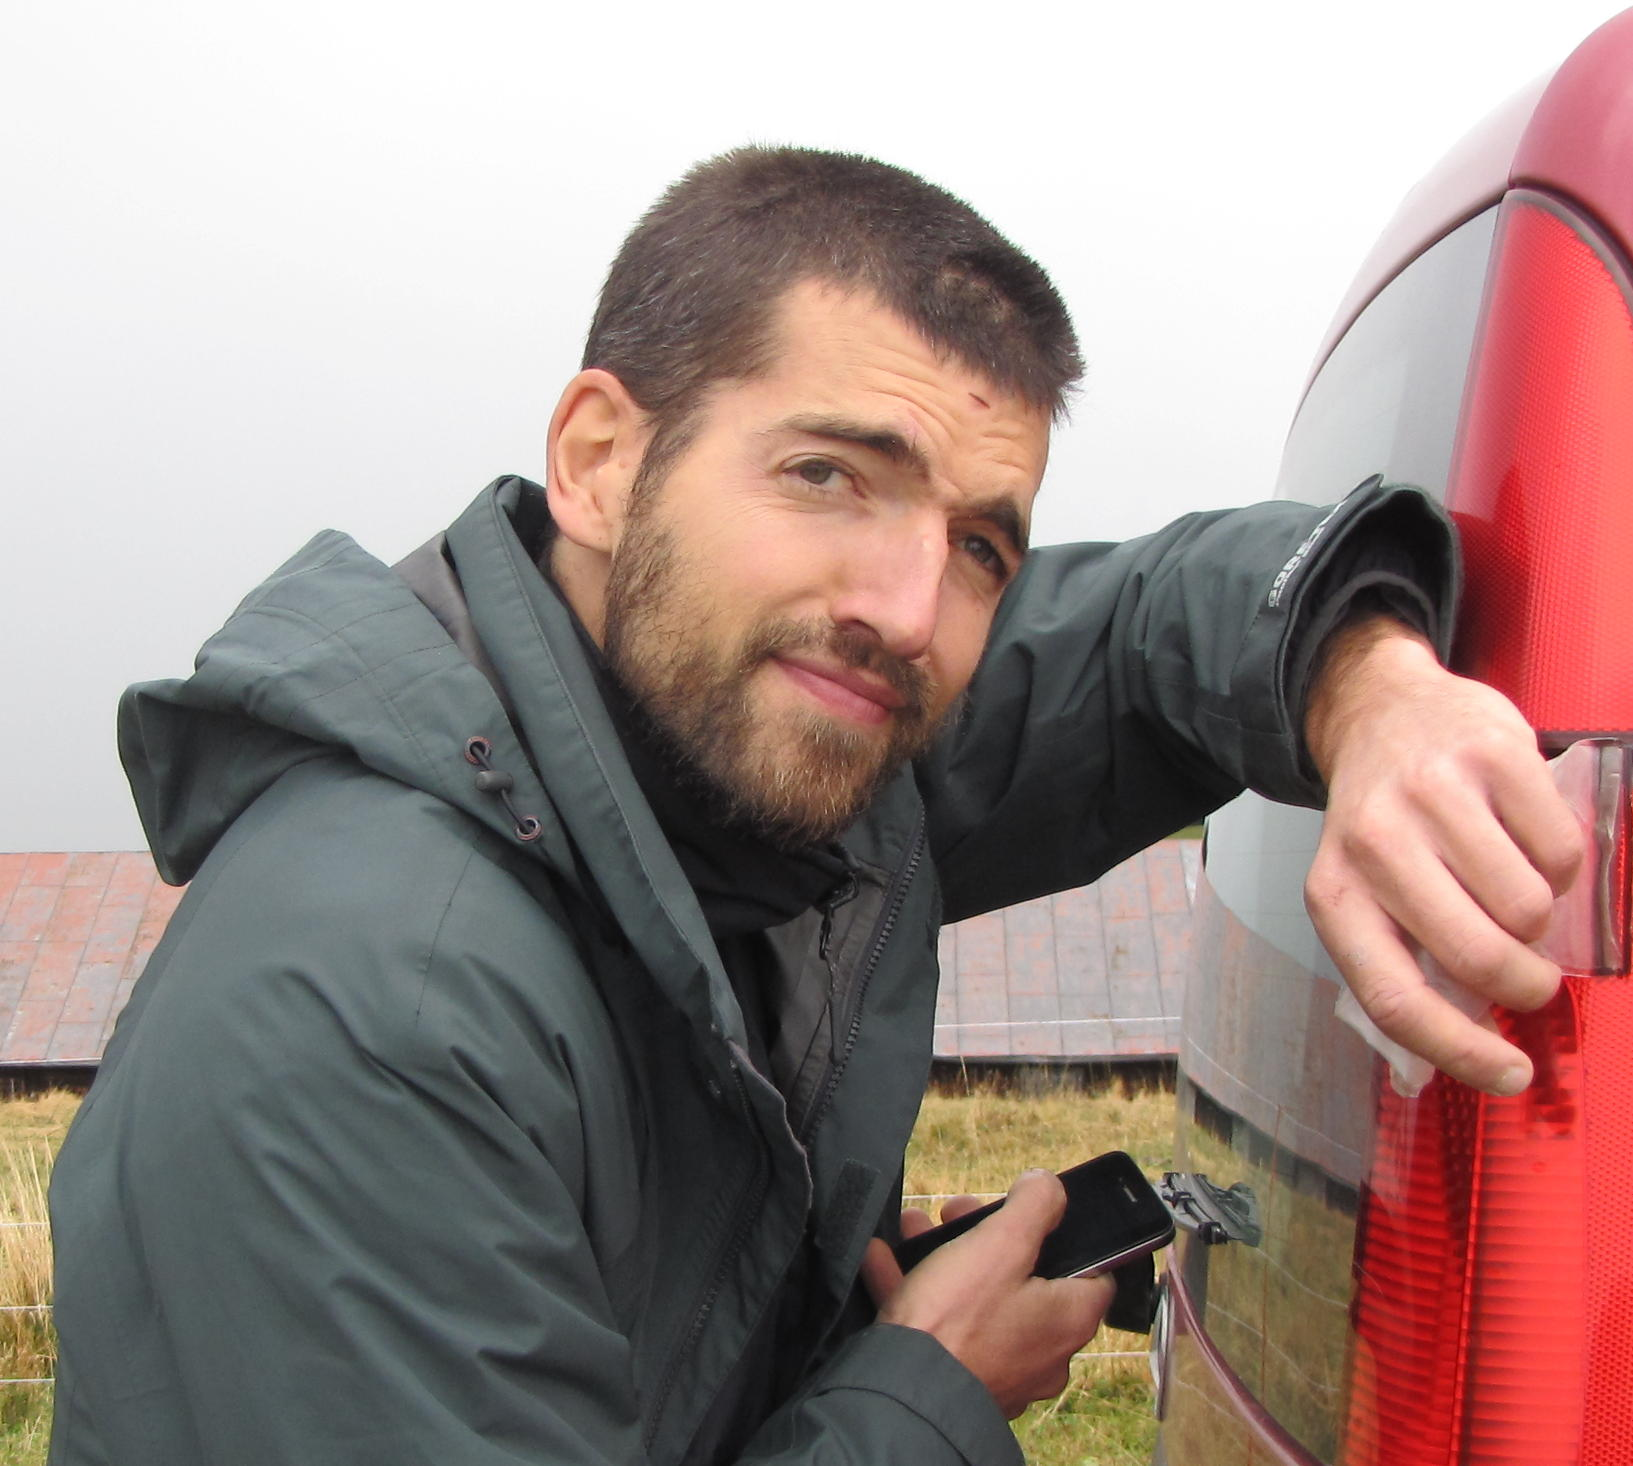
\includegraphics[width = 0.22 \textwidth]{Figures/Glauco}};}
				\uncover<5->{\node (ursina) at ($(glauco)+(1.2,0)$) {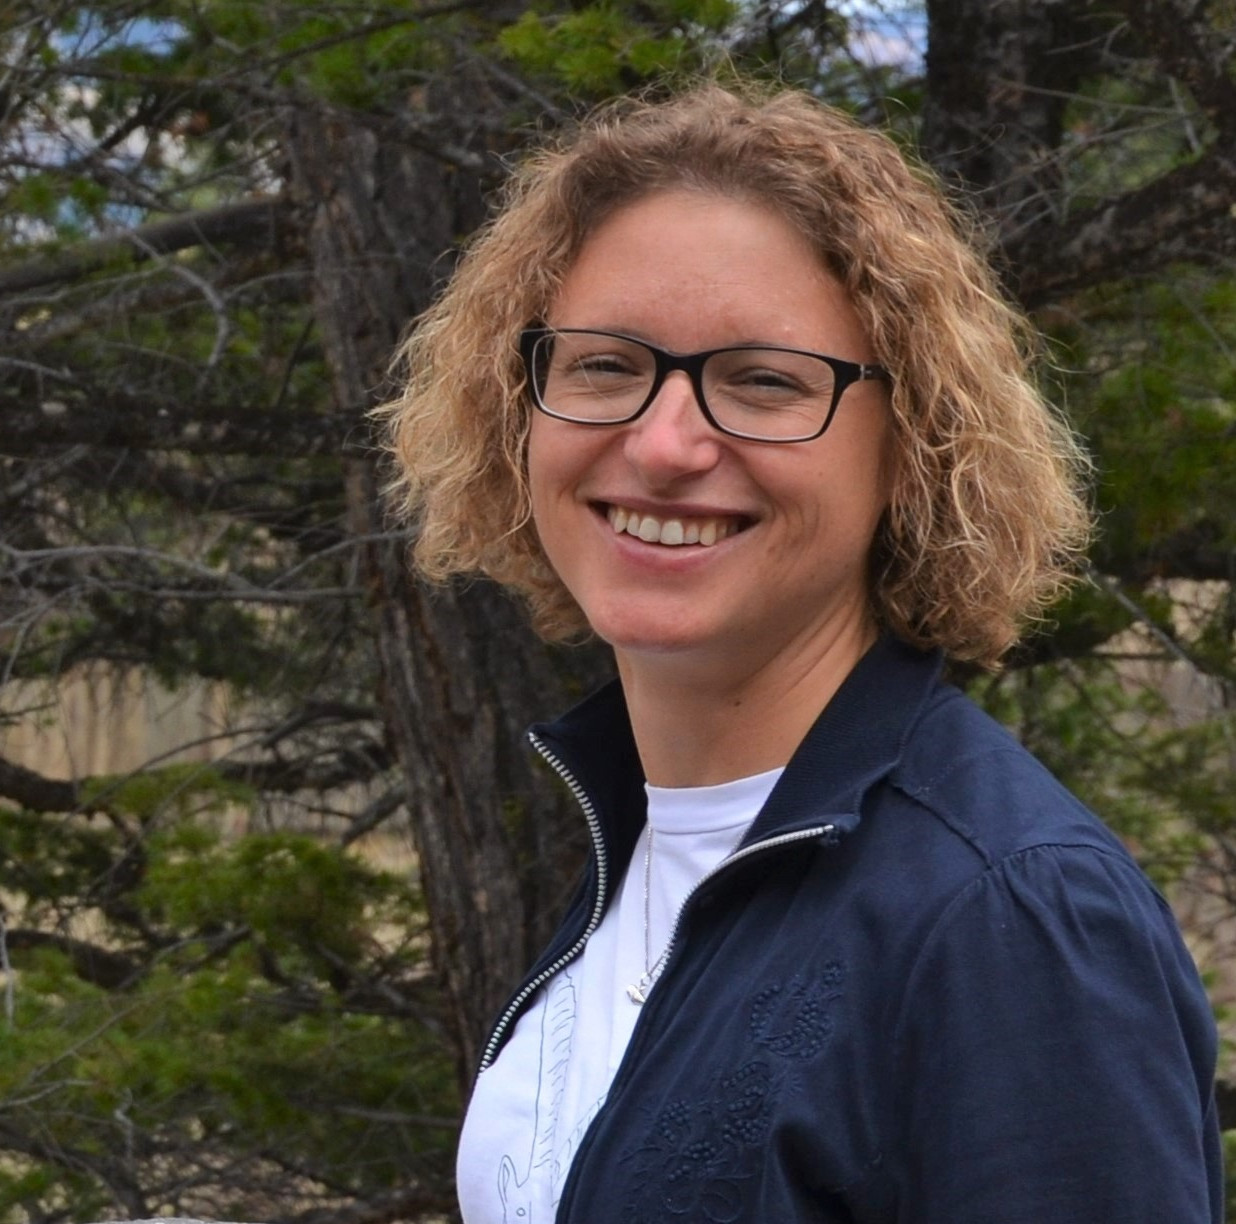
\includegraphics[width = 0.20 \textwidth]{Figures/Ursina}};}
				\uncover<6->{\node (domi) at ($(ursina)+(1.4,0)$) {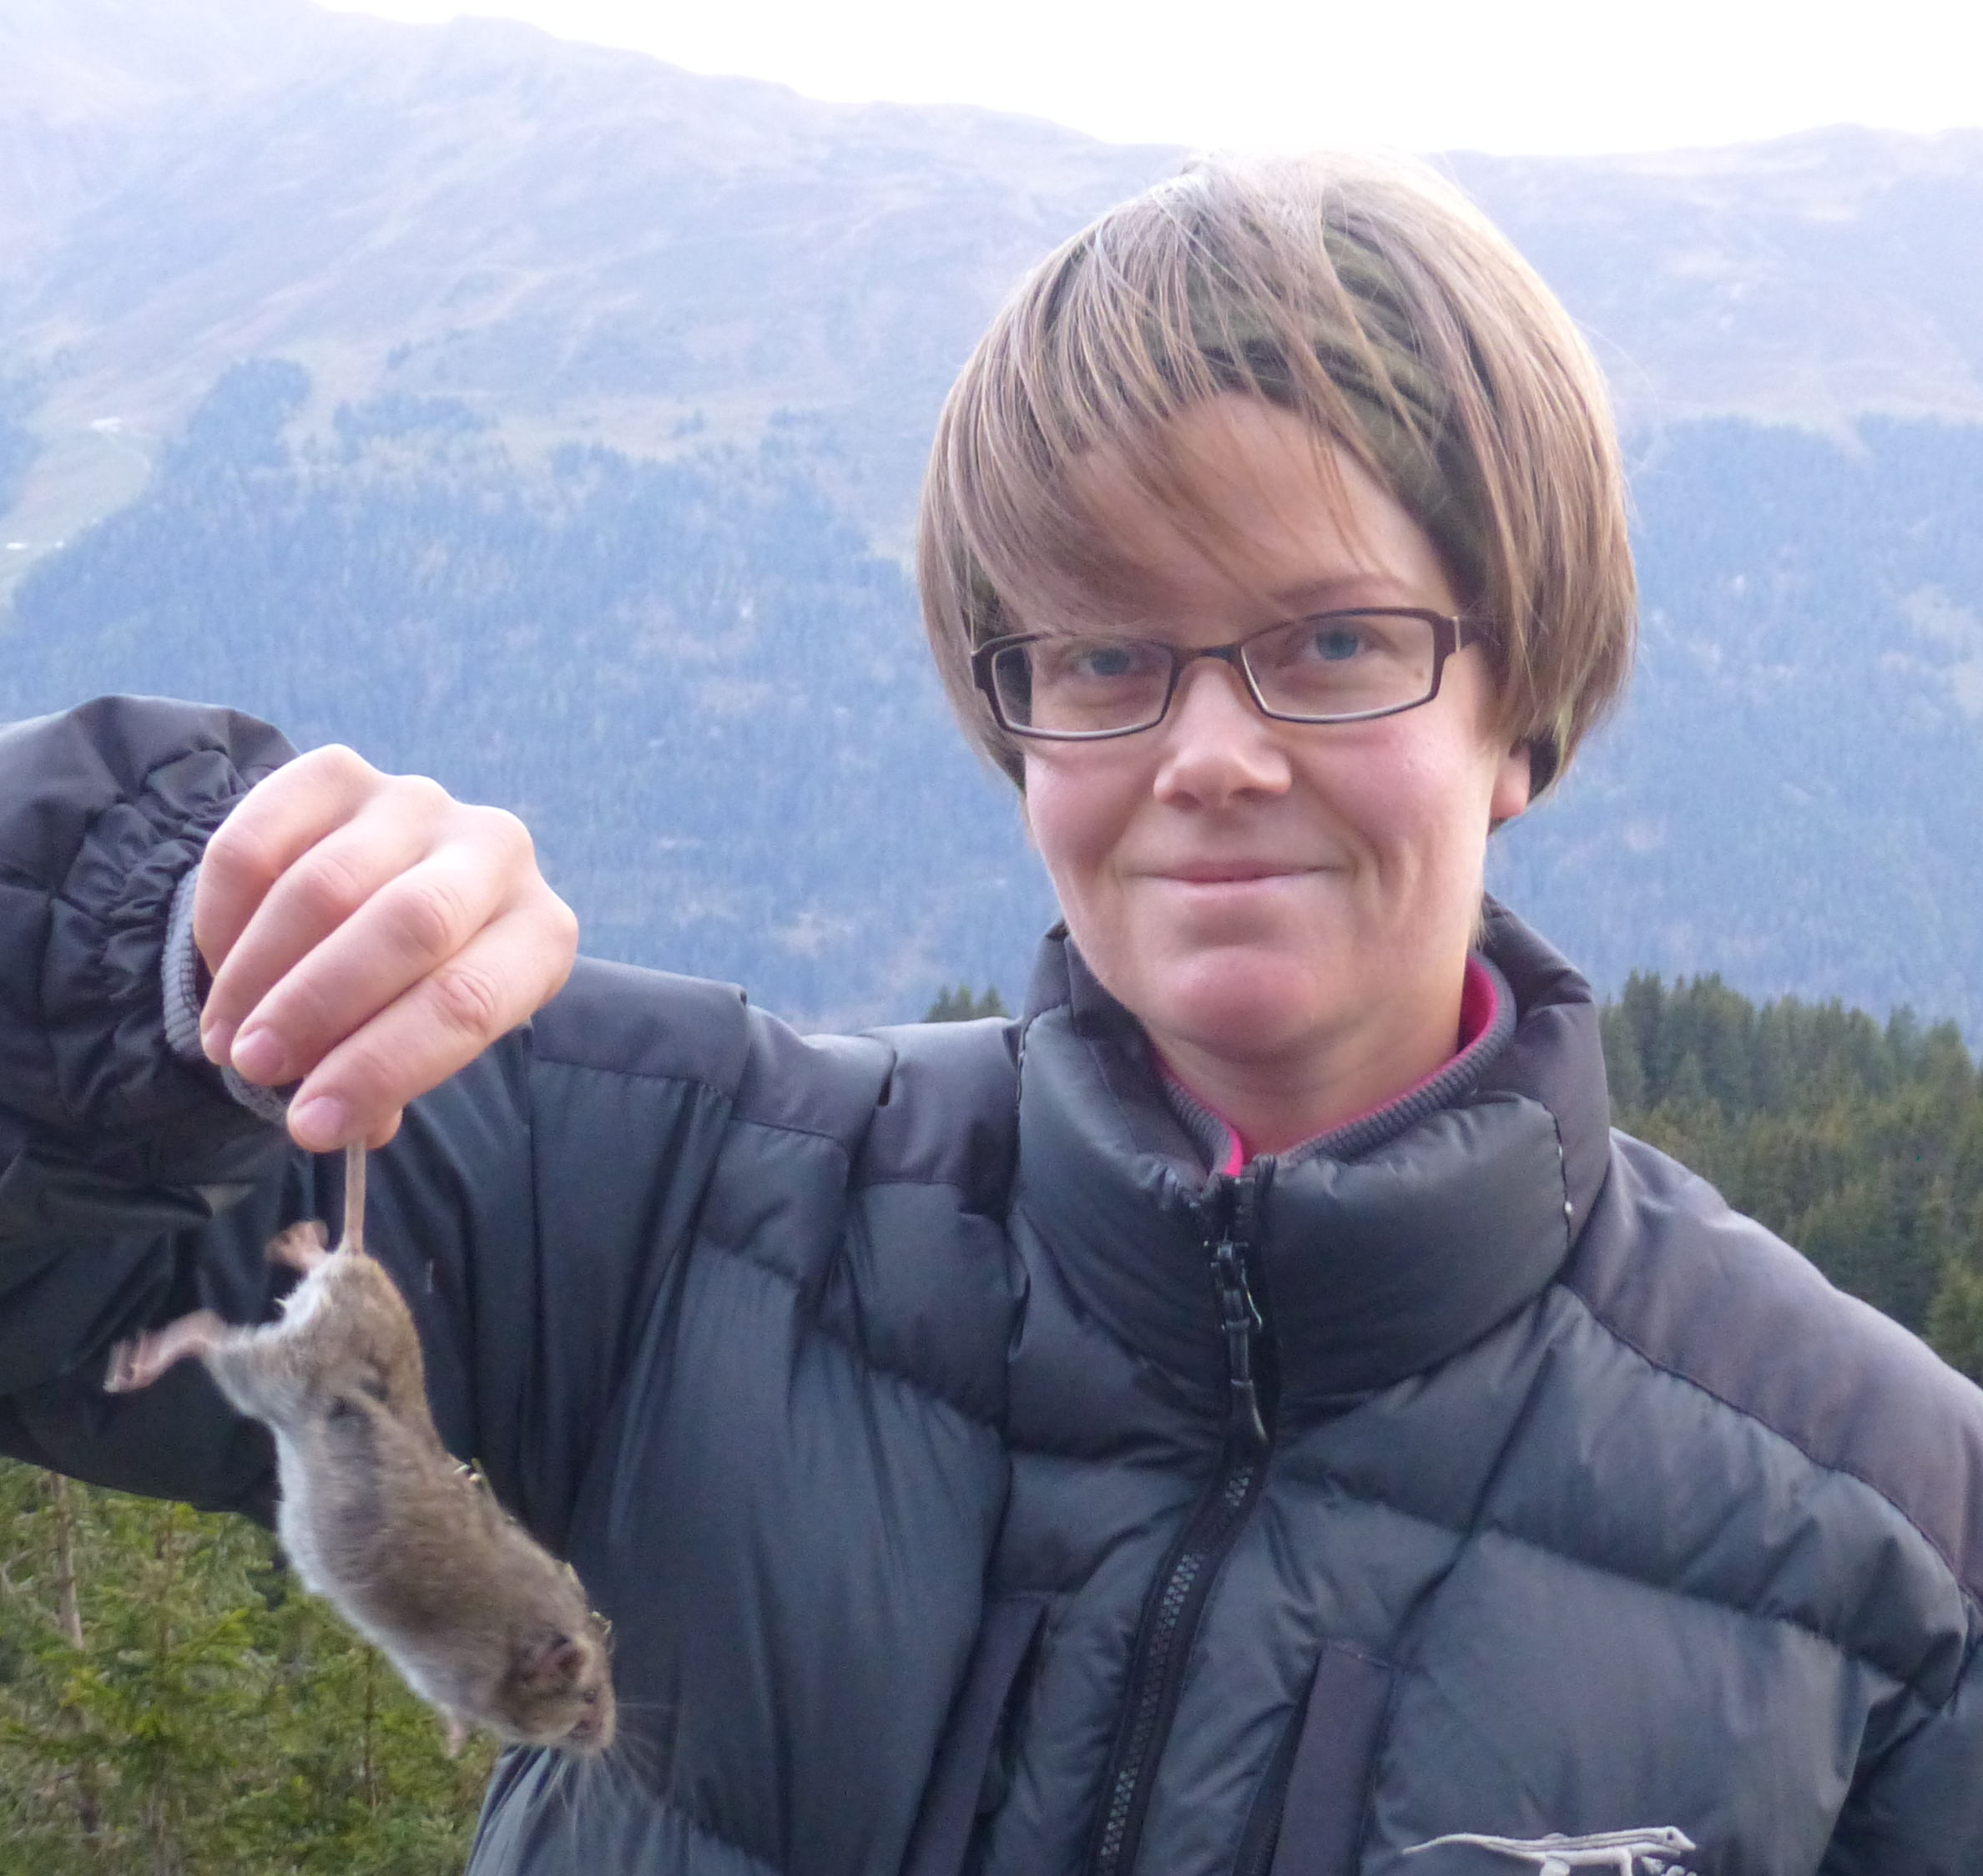
\includegraphics[width = 0.20 \textwidth]{Figures/Domi}};}
				\uncover<6->{\node (martina) at ($(domi)+(1.2,0)$) {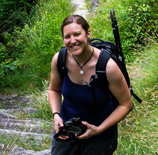
\includegraphics[width = 0.17 \textwidth]{Figures/Martina}};}
				\uncover<6->{\node (vicente) at ($(martina)+(1.2,-0.2)$) {\includegraphics[width = 0.16 \textwidth]{Figures/Vicente}};}
				\uncover<7->{\node (andres) at ($(vicente)+(1.2,-0.1)$) {\includegraphics[width = 0.2 \textwidth]{Figures/Andres}};}
				\uncover<8->{\node (koen) at ($(glauco)+(0,-1.4)$) {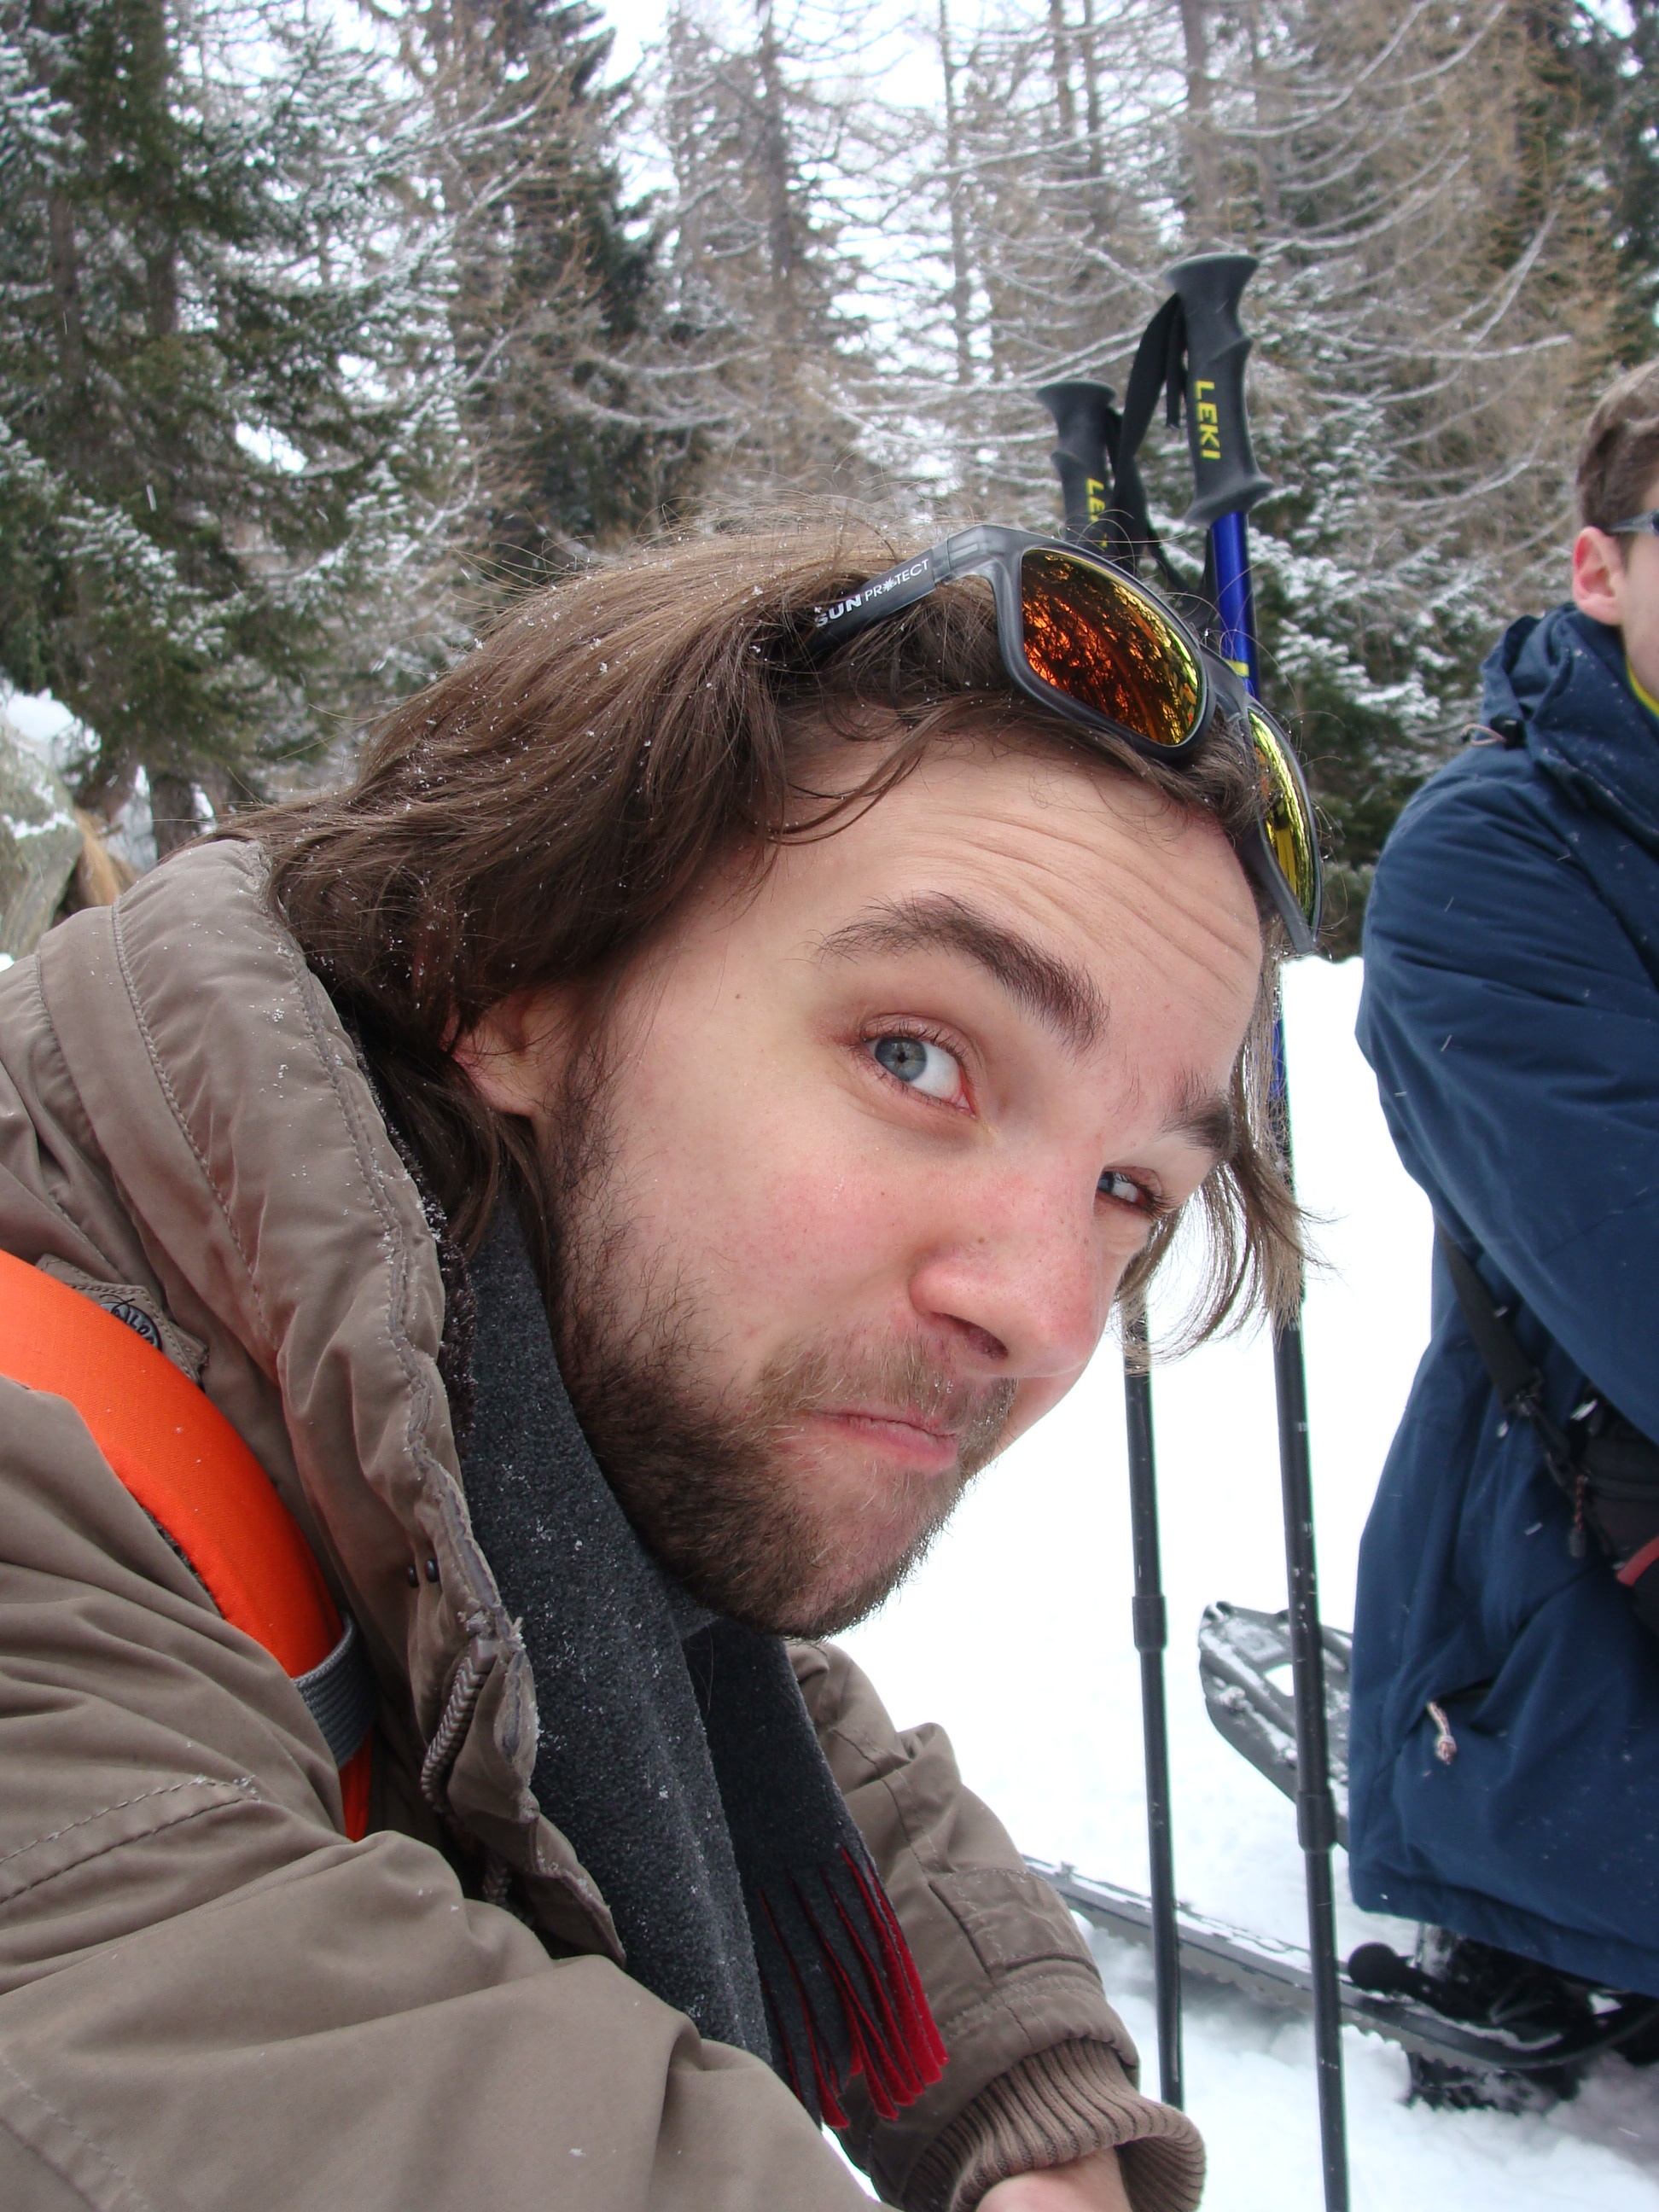
\includegraphics[width = 0.2 \textwidth]{Figures/Koen}};
				\node (marjolein) at ($(koen)+(1.2,0)$) {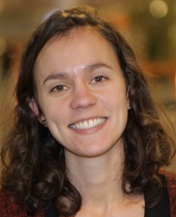
\includegraphics[width = 0.15 \textwidth]{Figures/Marjolein}};
				\node (eelke) at ($(marjolein)+(1.2,0)$) {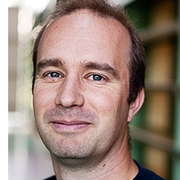
\includegraphics[width = 0.2 \textwidth]{Figures/Eelke}};
				}
				\uncover<9->{
				
				\node (philipp) at ($(eelke)+(1.2,0)$) {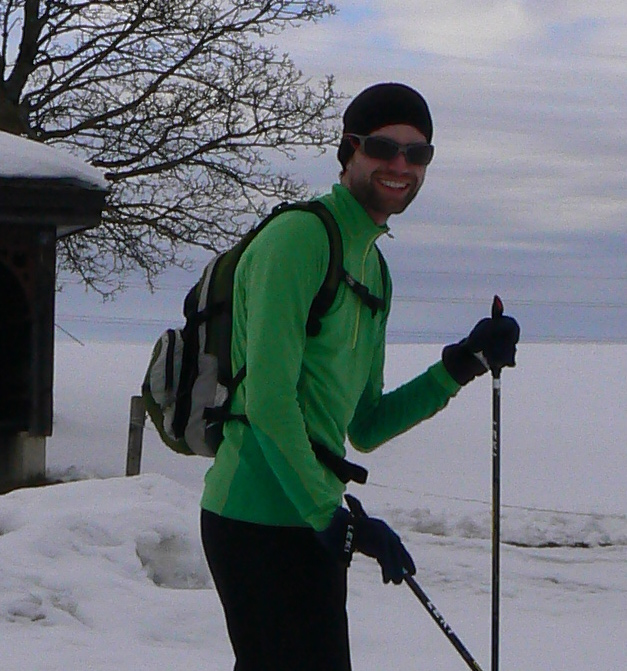
\includegraphics[width = 0.2 \textwidth]{Figures/Philipp}};
				\node (pirmin) at ($(philipp)+(1.2,0)$) {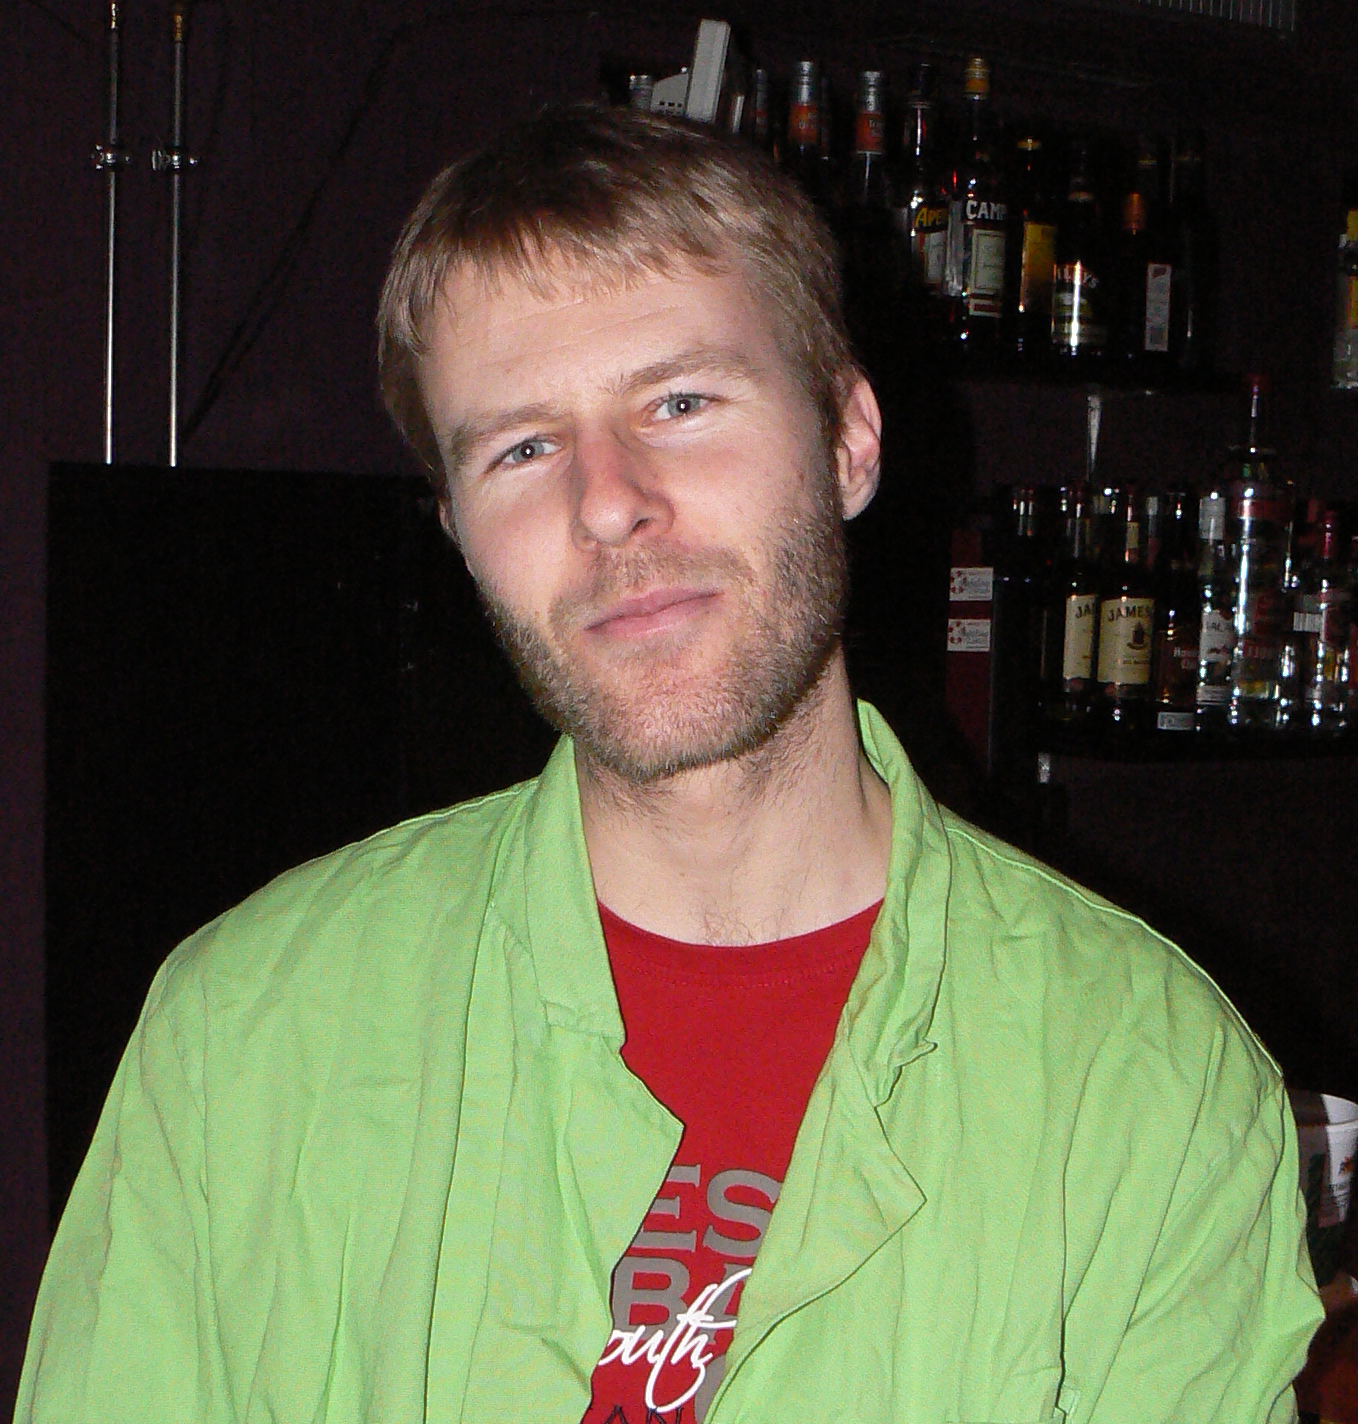
\includegraphics[width = 0.2 \textwidth]{Figures/Pirmin}};
				\node (judith) at ($(pirmin)+(1.2,0)$) {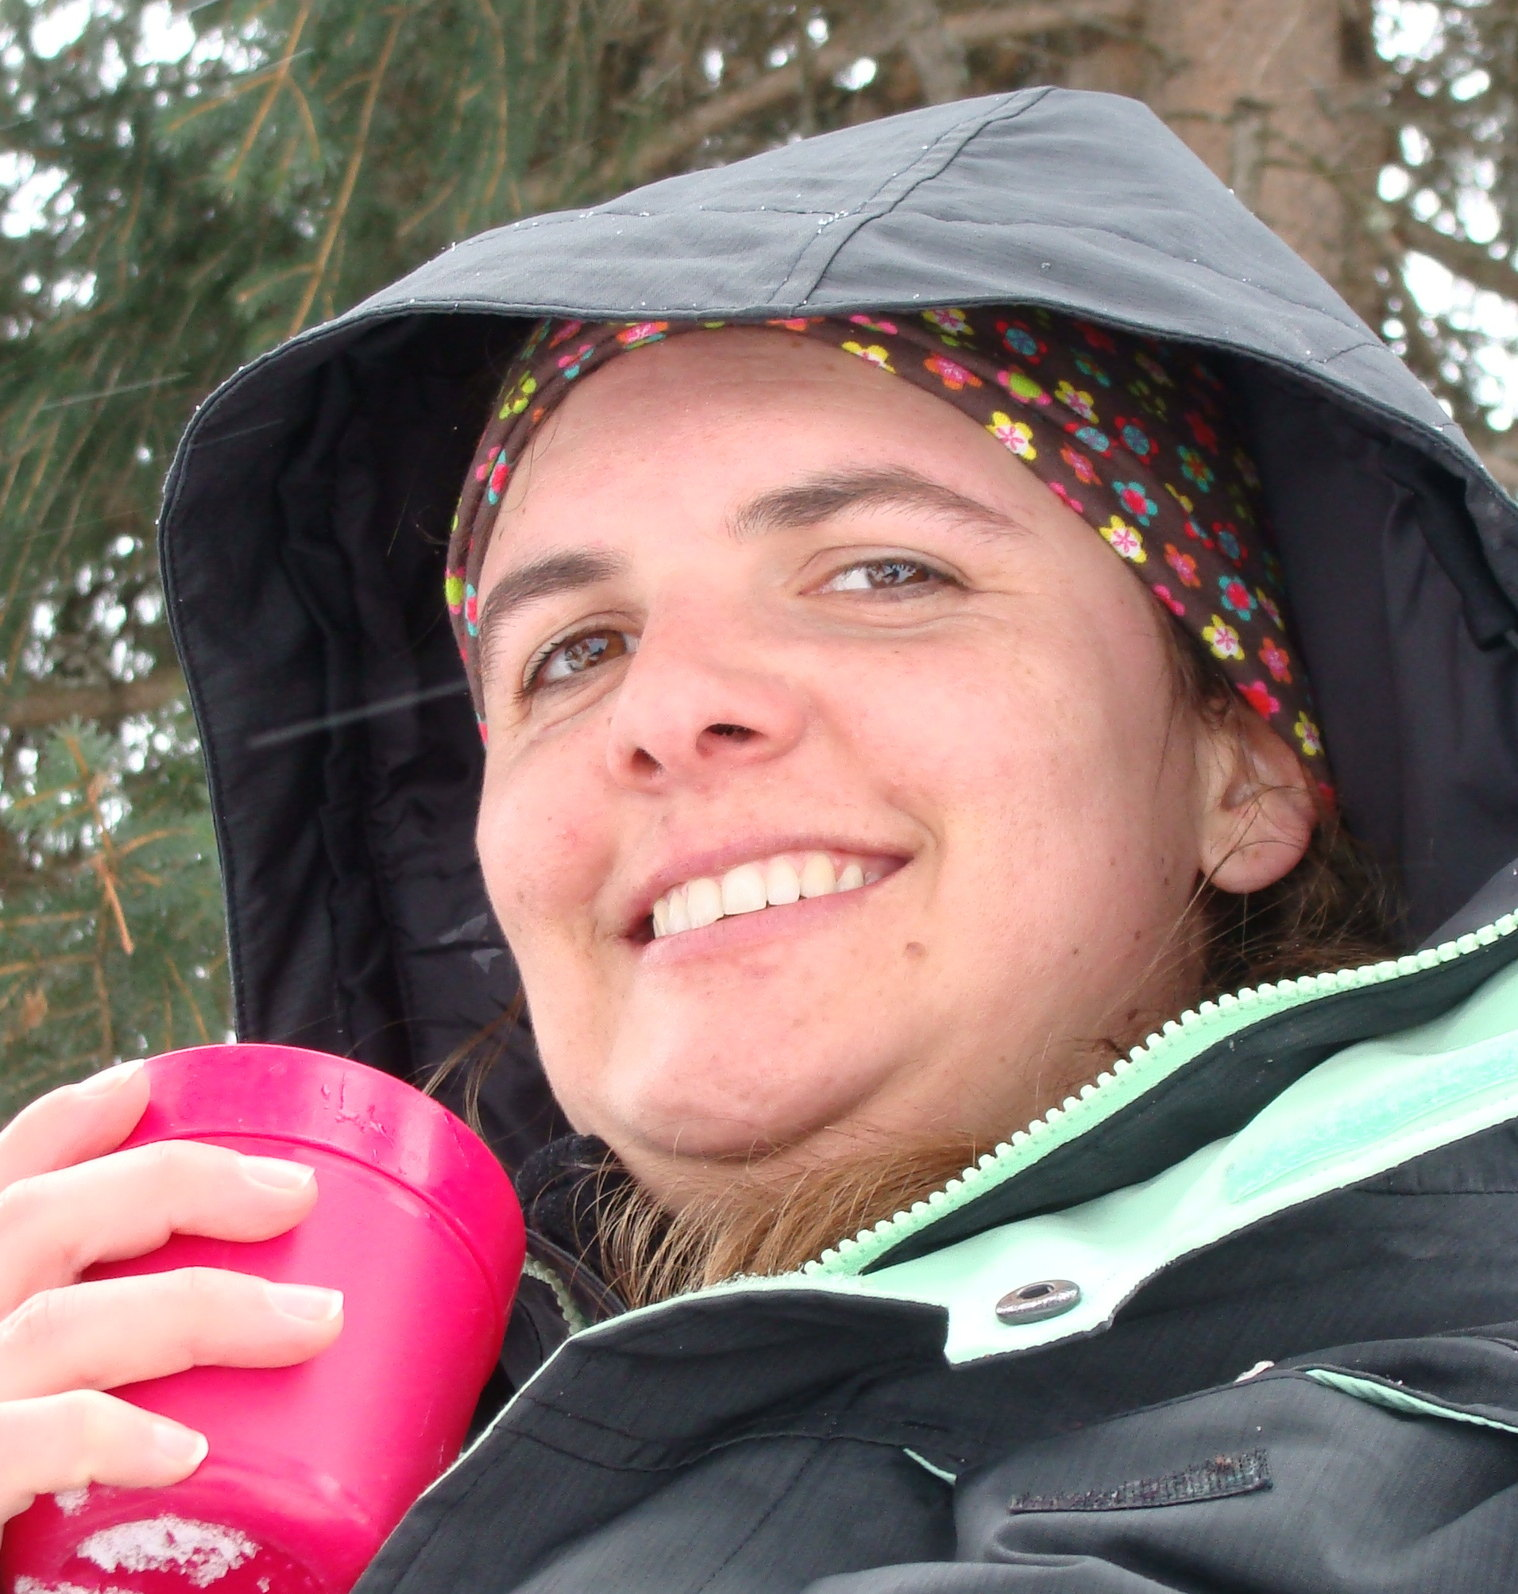
\includegraphics[width = 0.18 \textwidth]{Figures/Judith}};
				}
					\end{tikzpicture}
		\end{figure}
	\end{column}
\end{columns}

\end{frame}
%%%%%%%%%%%

\begin{frame}[plain]
\begin{columns}
\begin{column}[c]{0.7\textwidth}
		\begin{figure}[c]
			\begin{tikzpicture}

							\node (erik) at (0,0) {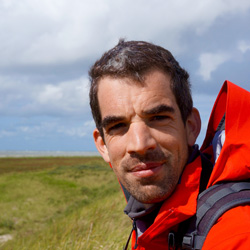
\includegraphics[width = 0.2 \textwidth]{Figures/Erik}};
				\node (lukas) at ($(erik)+(1.2,0)$) {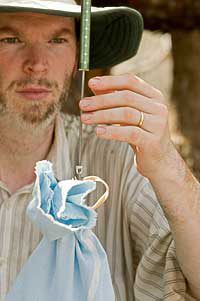
\includegraphics[width = 0.15 \textwidth]{Figures/Lukas}};
				\node (barbara) at ($(lukas)+(1,0)$) {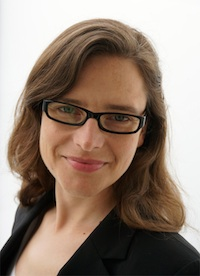
\includegraphics[width = 0.15 \textwidth]{Figures/Barbara}};
				\node (arpat) at ($(barbara)+(1.3,0)$) {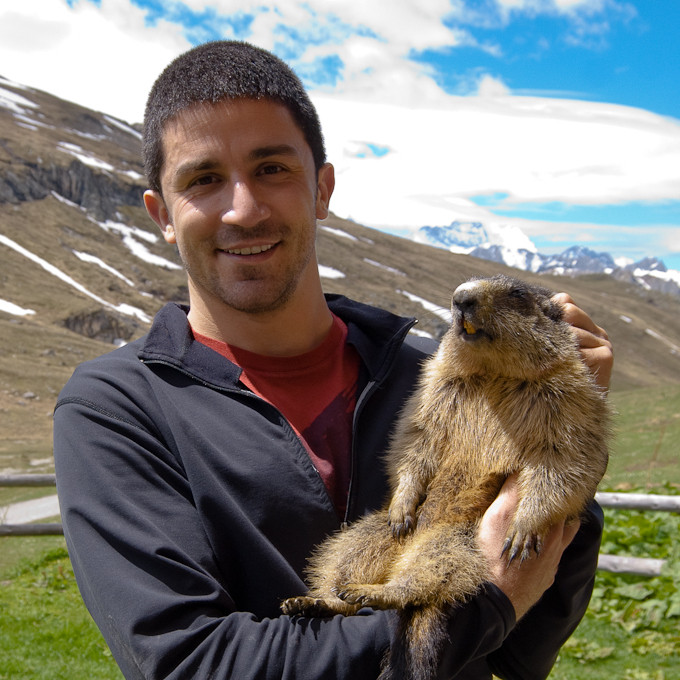
\includegraphics[width = 0.2 \textwidth]{Figures/Arpat}};
				\node (marc) at ($(arpat)+(1.2,0)$) {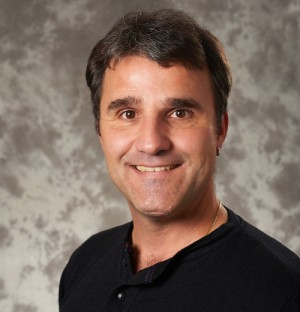
\includegraphics[width = 0.2 \textwidth]{Figures/Marc}};
				\node (jarrod) at ($(marc)+(1.3,0)$) {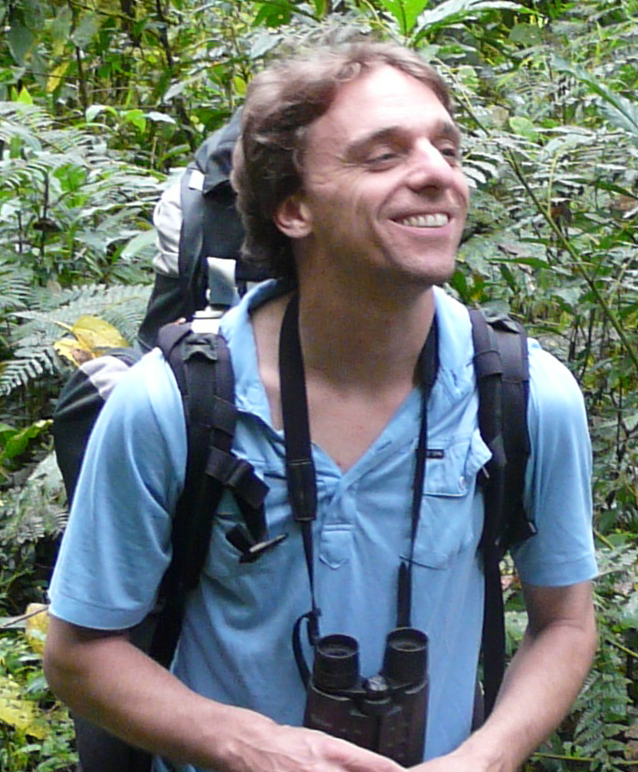
\includegraphics[width = 0.2\textwidth]{Figures/Jarrod}};
				\node (glauco) at ($(erik)+(0,-1.4)$) {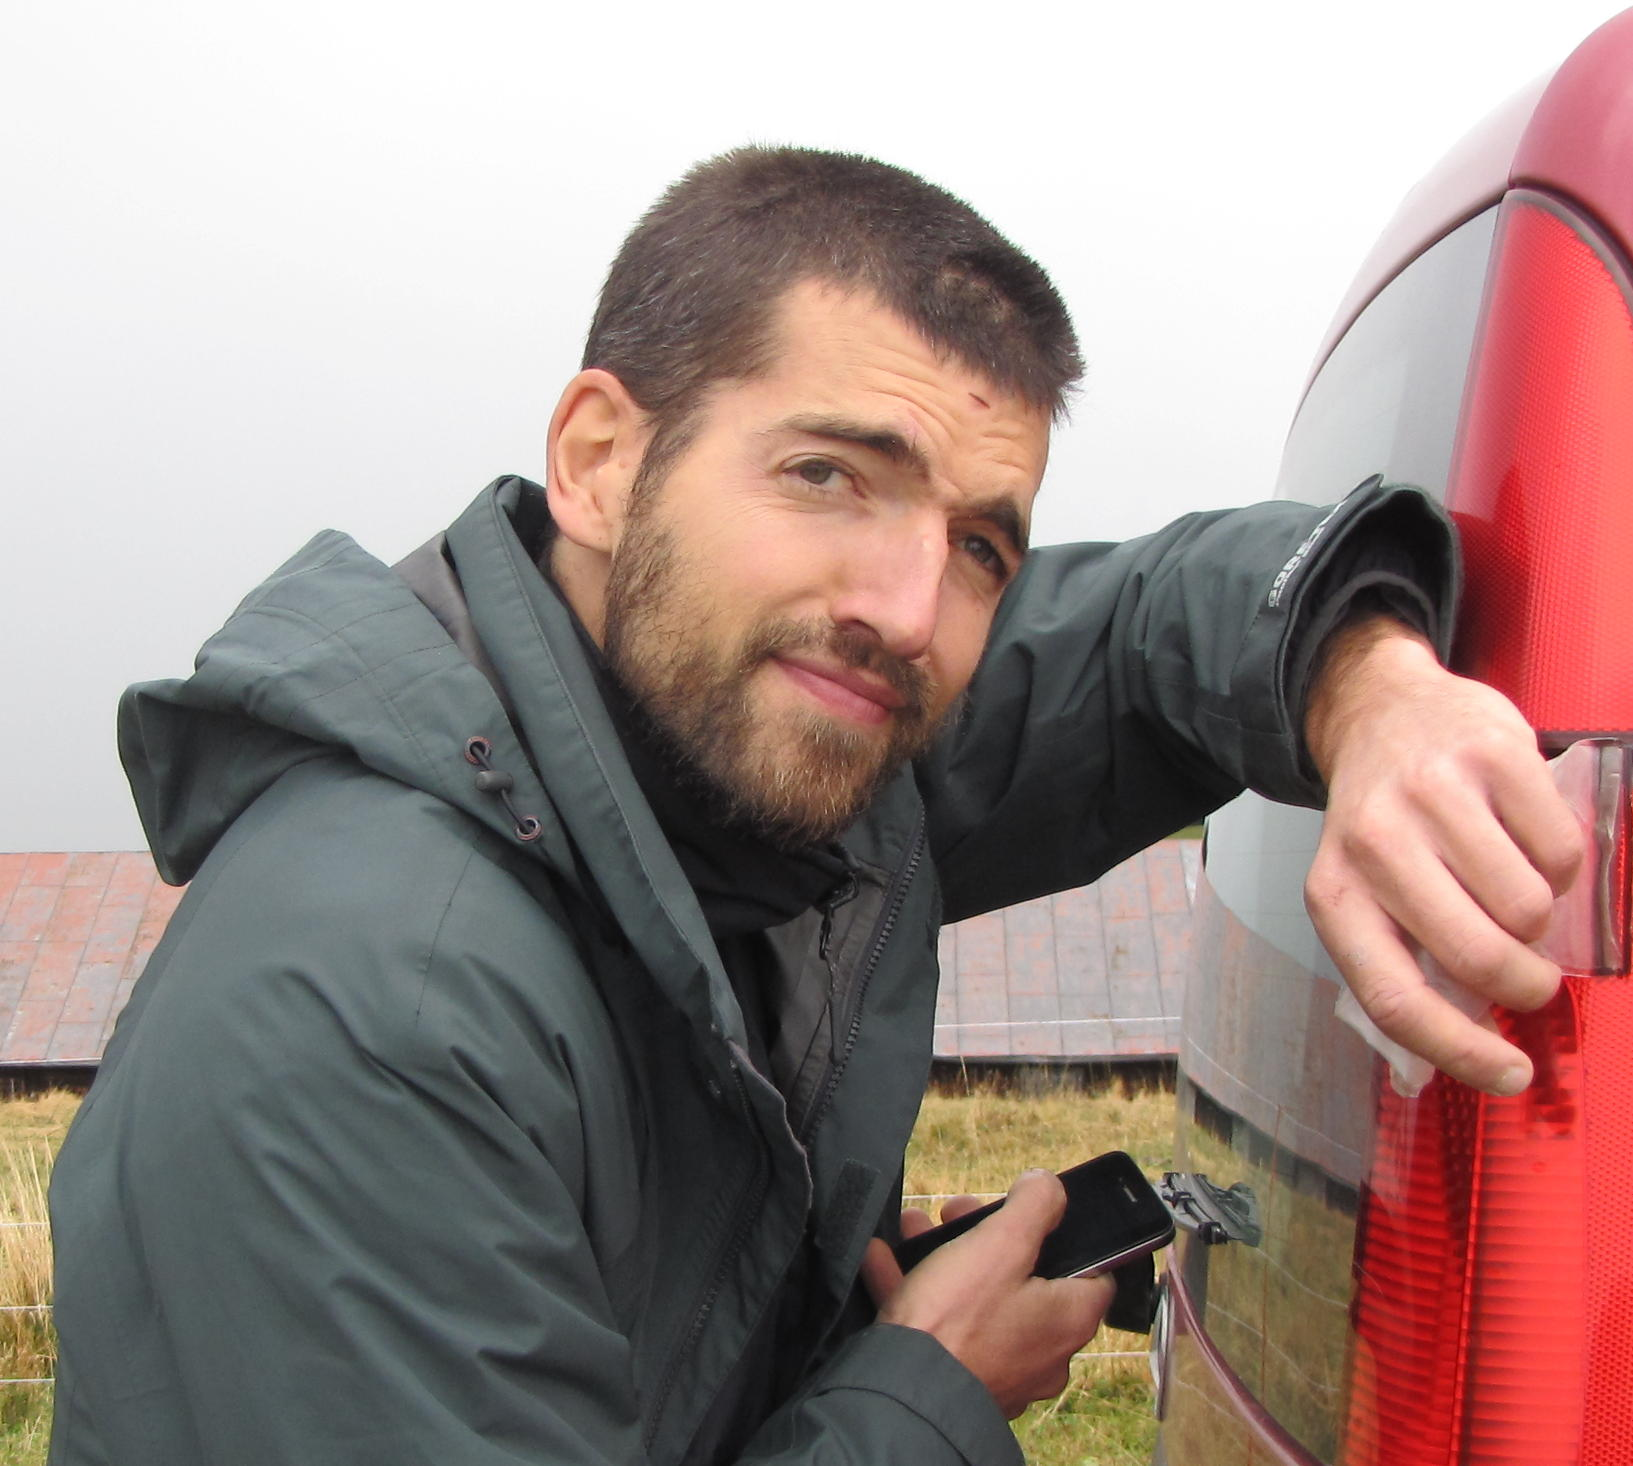
\includegraphics[width = 0.22 \textwidth]{Figures/Glauco}};
			\node (ursina) at ($(glauco)+(1.2,0)$) {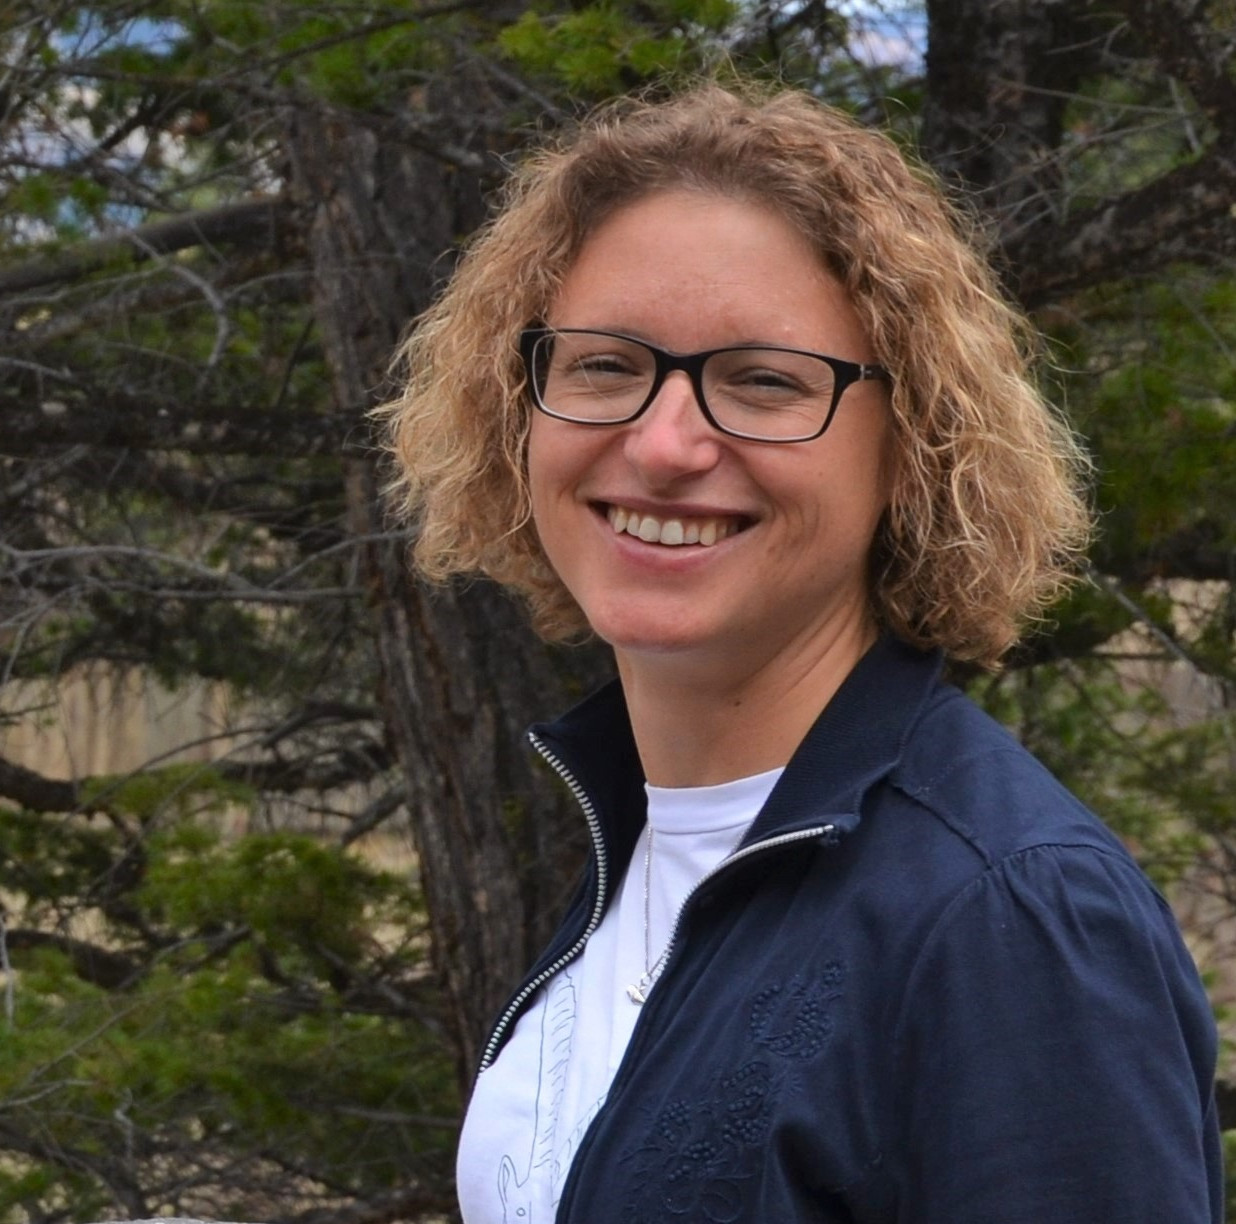
\includegraphics[width = 0.20 \textwidth]{Figures/Ursina}};
				\node (domi) at ($(ursina)+(1.4,0)$) {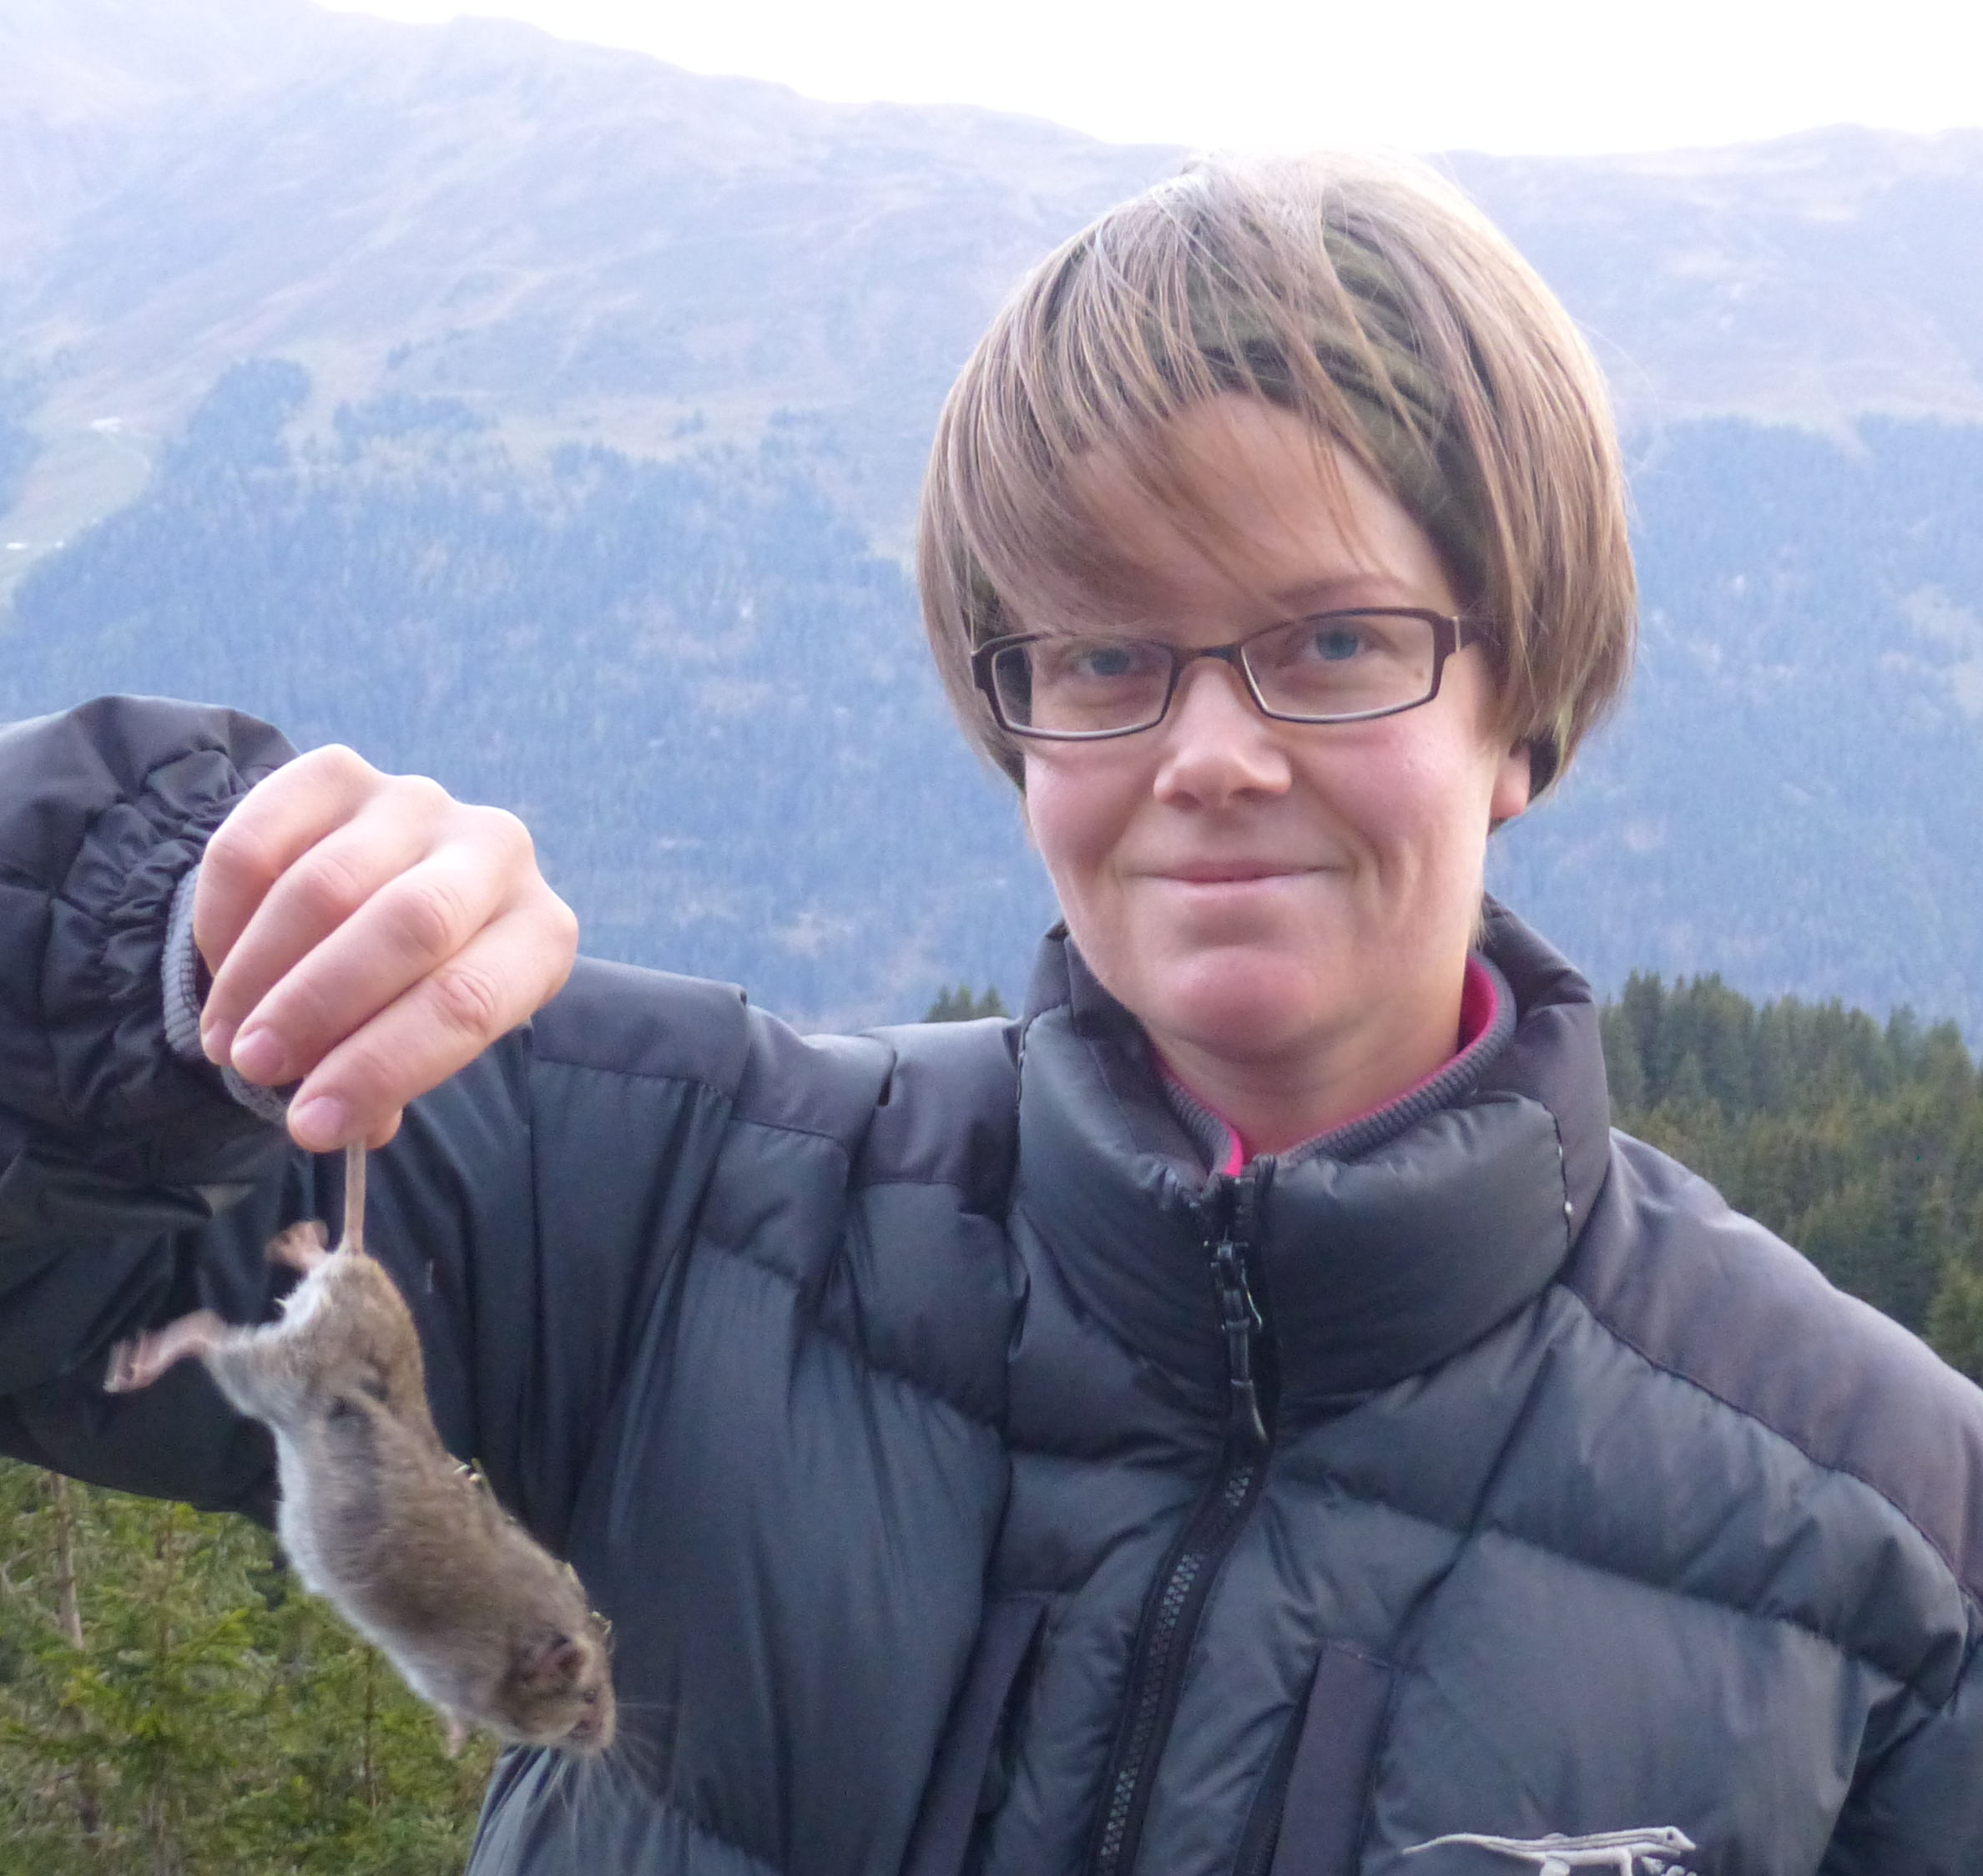
\includegraphics[width = 0.20 \textwidth]{Figures/Domi}};
				\node (martina) at ($(domi)+(1.2,0)$) {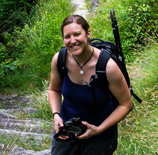
\includegraphics[width = 0.17 \textwidth]{Figures/Martina}};
\node (vicente) at ($(martina)+(1.2,-0.2)$) {\includegraphics[width = 0.16 \textwidth]{Figures/Vicente}};
	\node (andres) at ($(vicente)+(1.2,-0.1)$) {\includegraphics[width = 0.2 \textwidth]{Figures/Andres}};
\node (koen) at ($(glauco)+(0,-1.4)$) {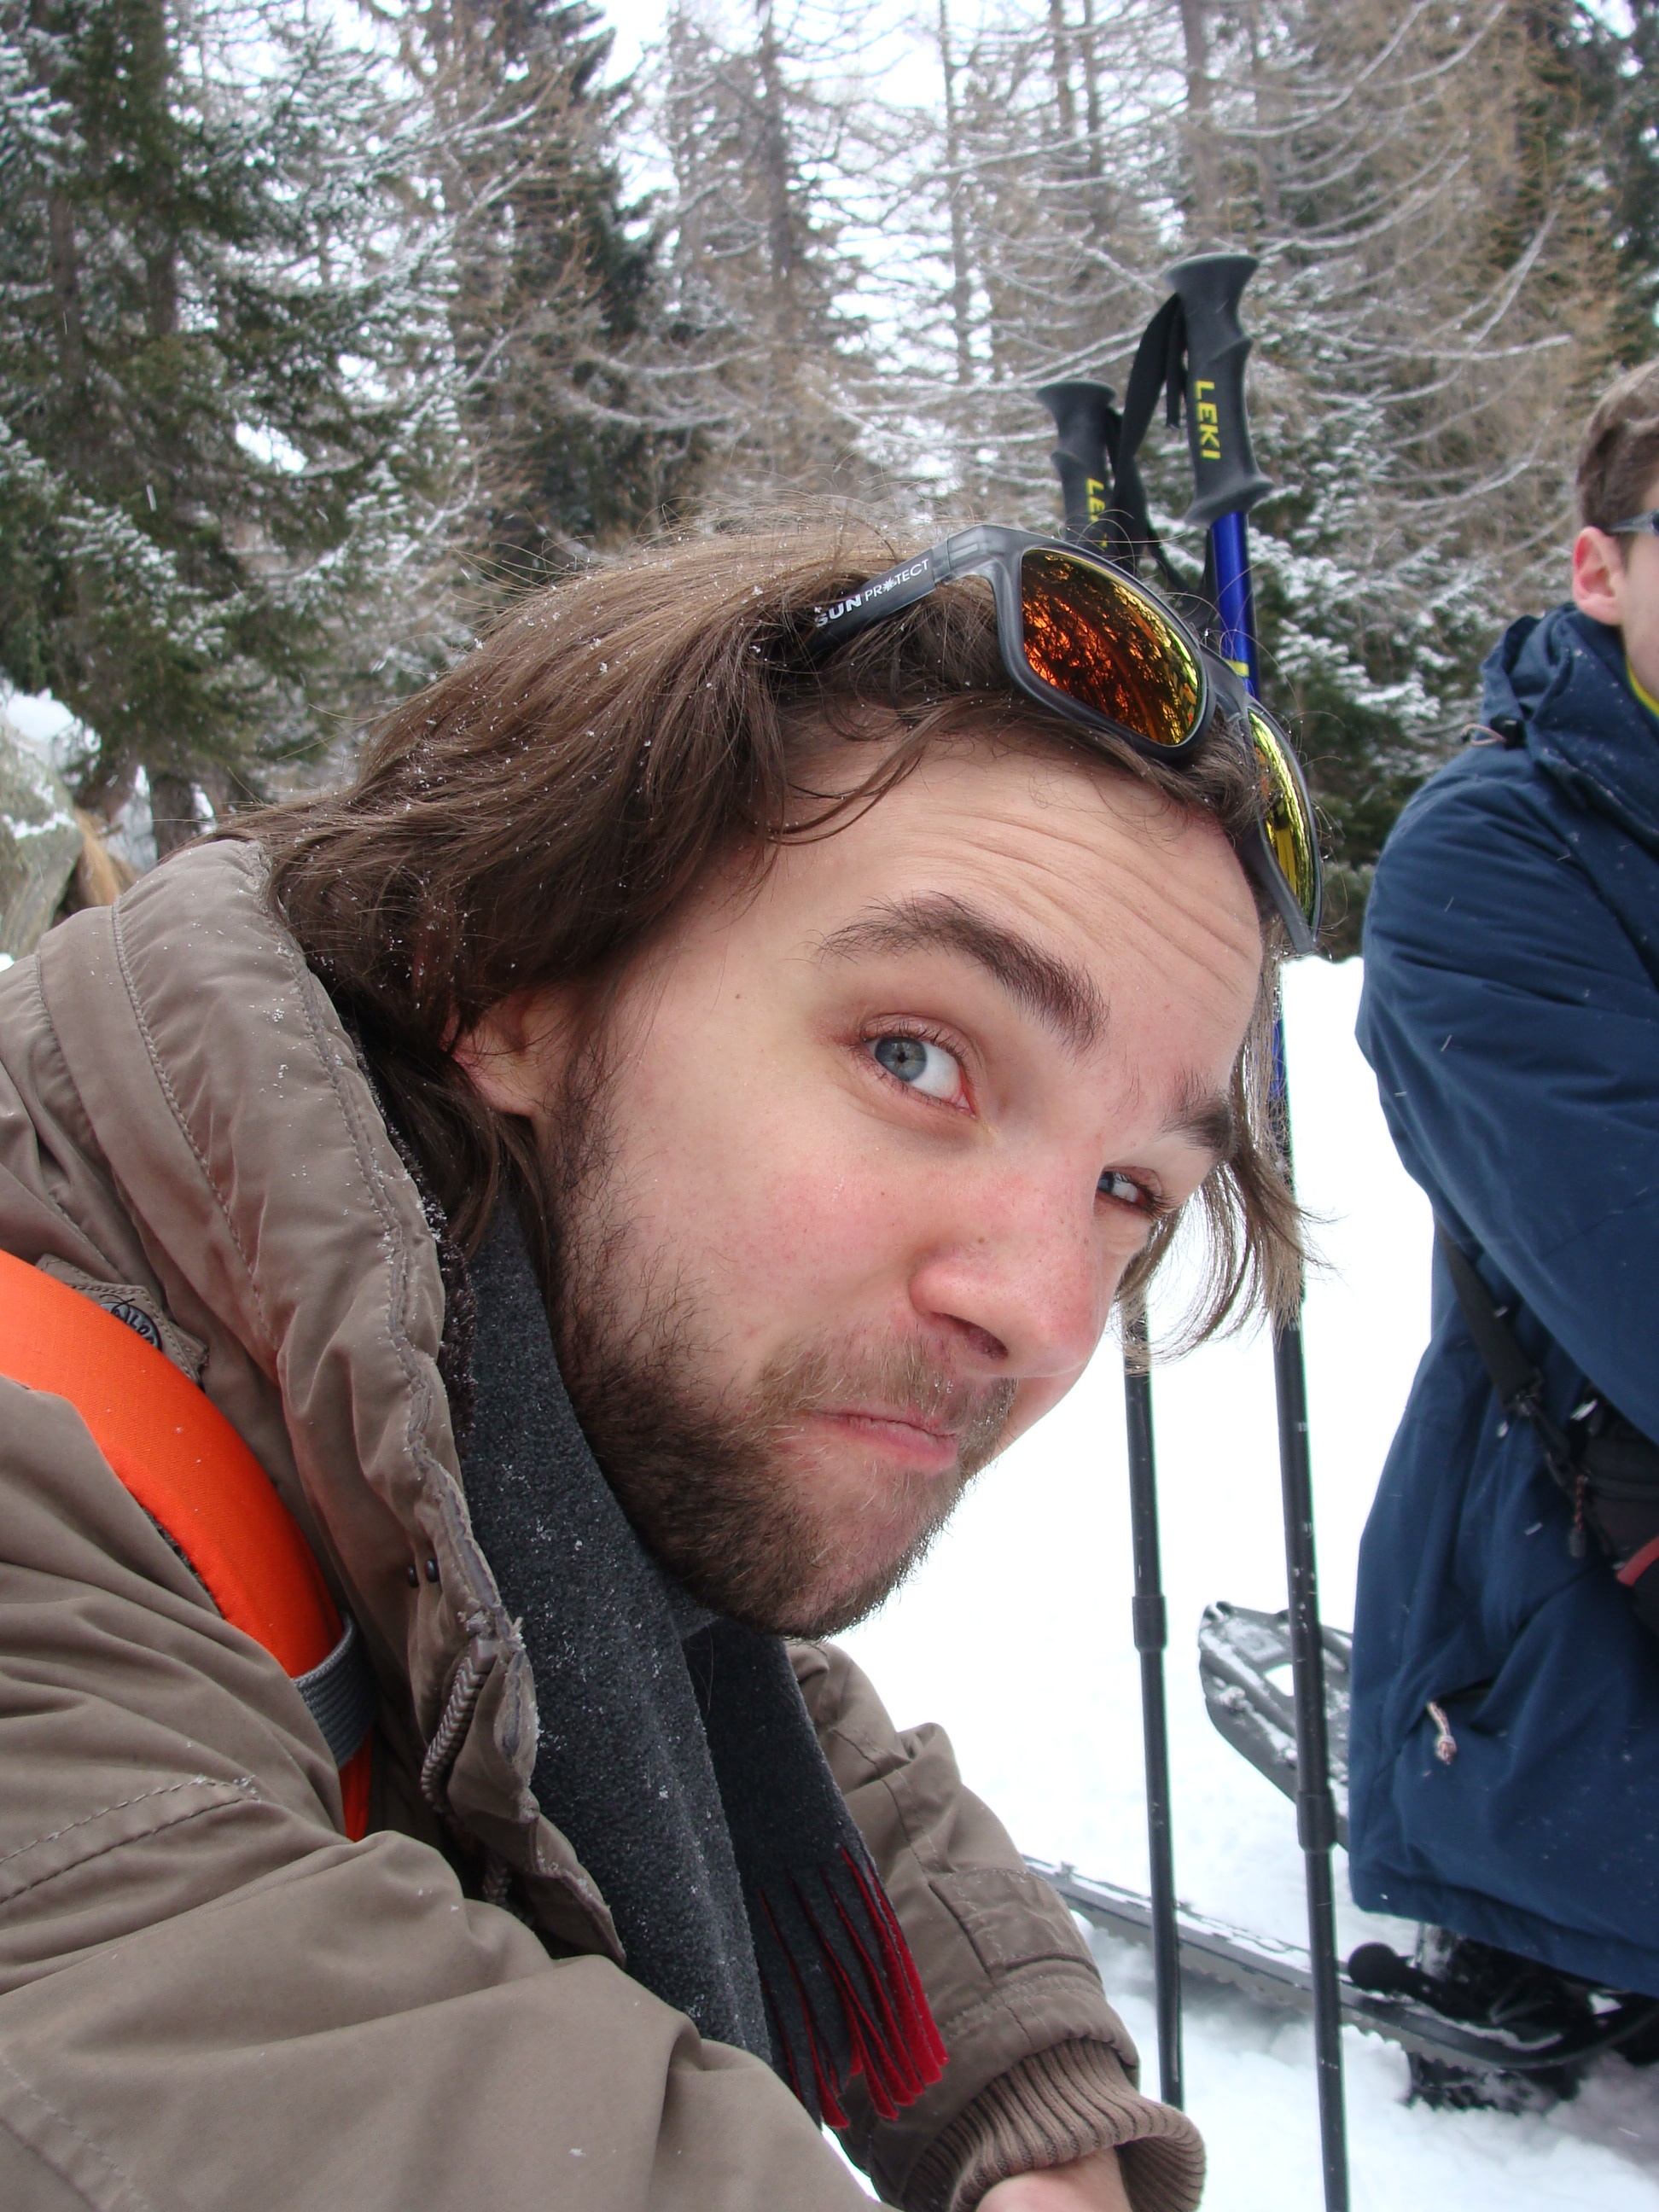
\includegraphics[width = 0.2 \textwidth]{Figures/Koen}};
				\node (marjolein) at ($(koen)+(1.2,0)$) {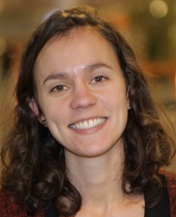
\includegraphics[width = 0.15 \textwidth]{Figures/Marjolein}};
				\node (eelke) at ($(marjolein)+(1.2,0)$) {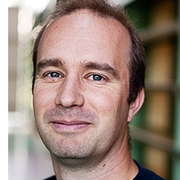
\includegraphics[width = 0.2 \textwidth]{Figures/Eelke}};
				
				
				\node (philipp) at ($(eelke)+(1.2,0)$) {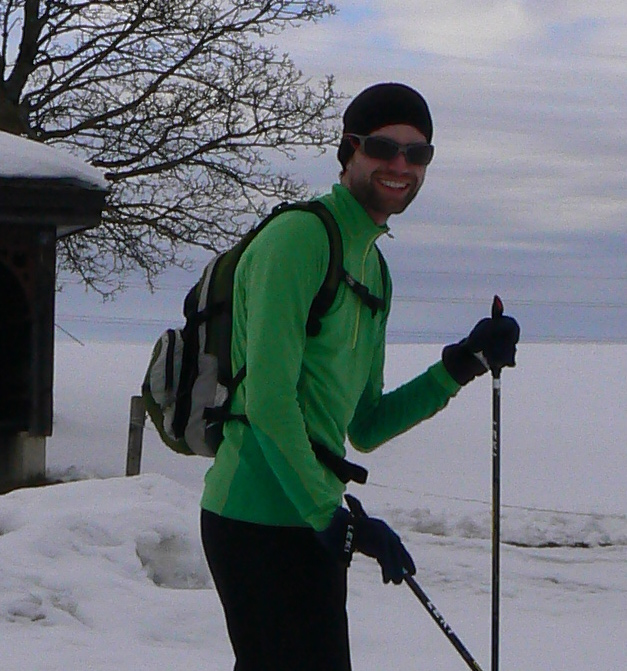
\includegraphics[width = 0.2 \textwidth]{Figures/Philipp}};
				\node (pirmin) at ($(philipp)+(1.2,0)$) {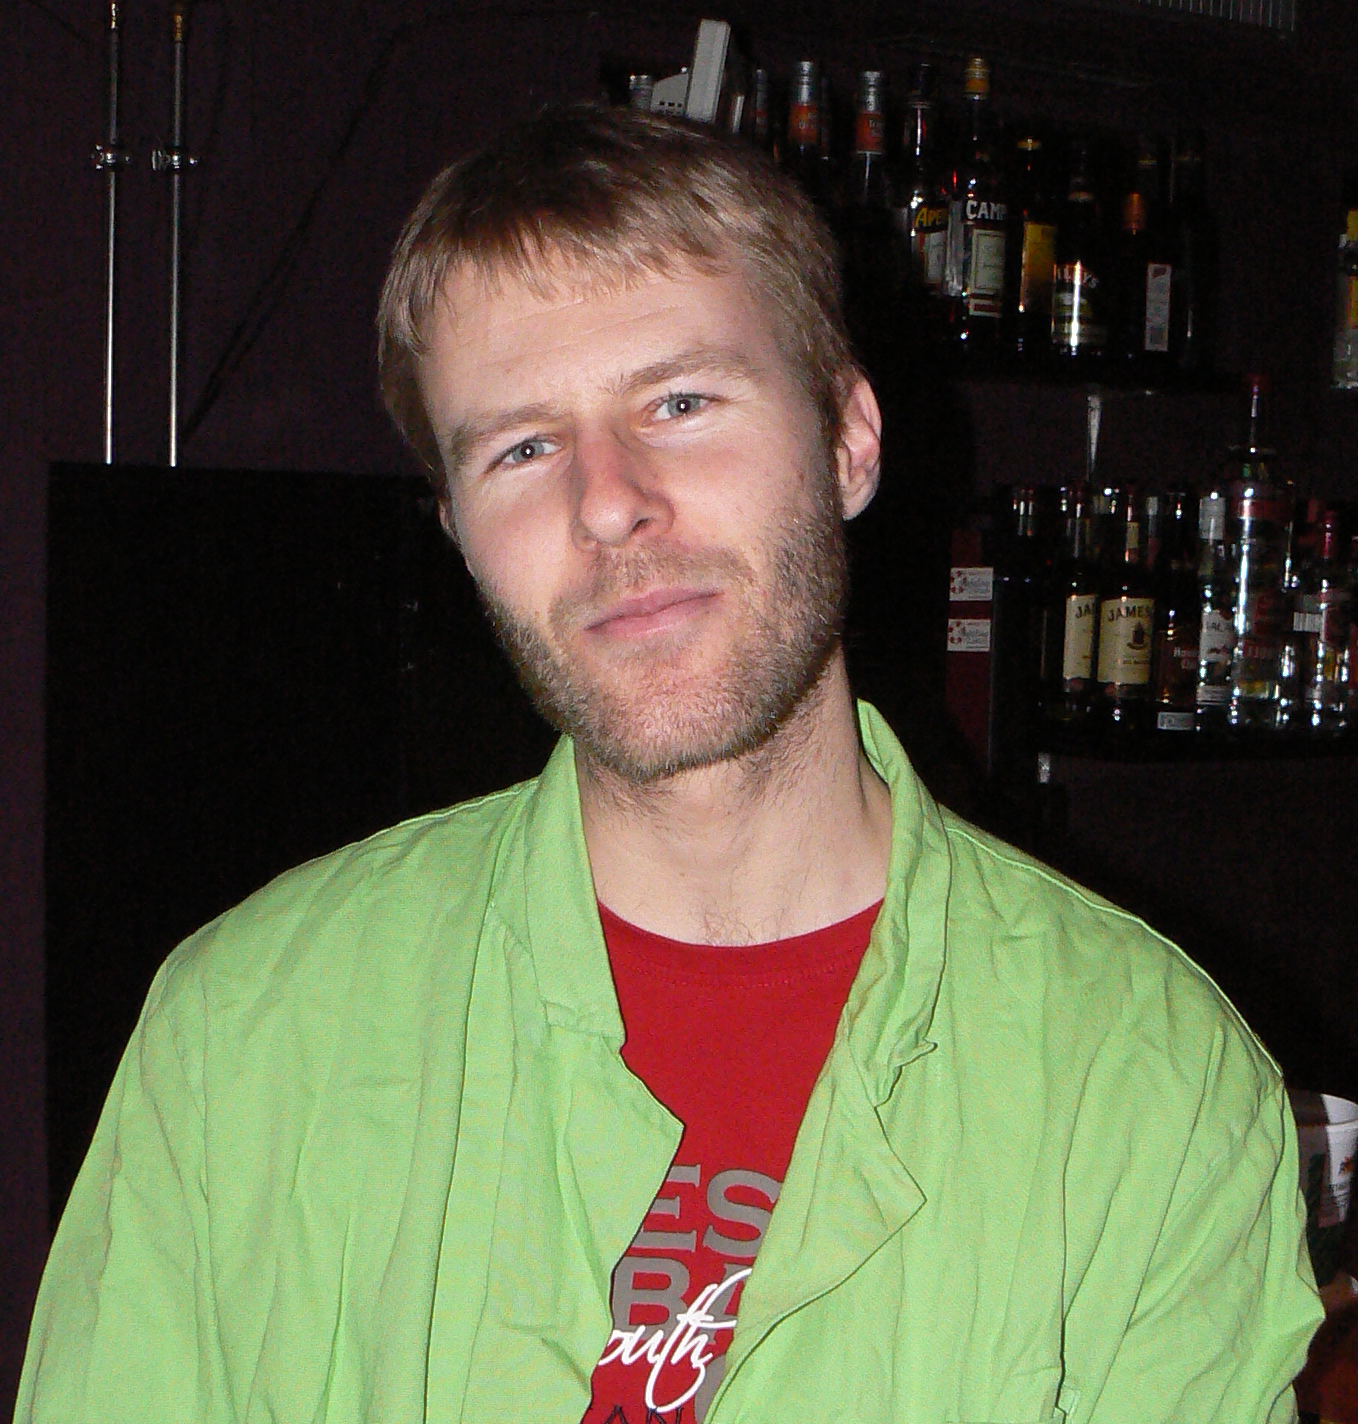
\includegraphics[width = 0.2 \textwidth]{Figures/Pirmin}};
				\node (judith) at ($(pirmin)+(1.2,0)$) {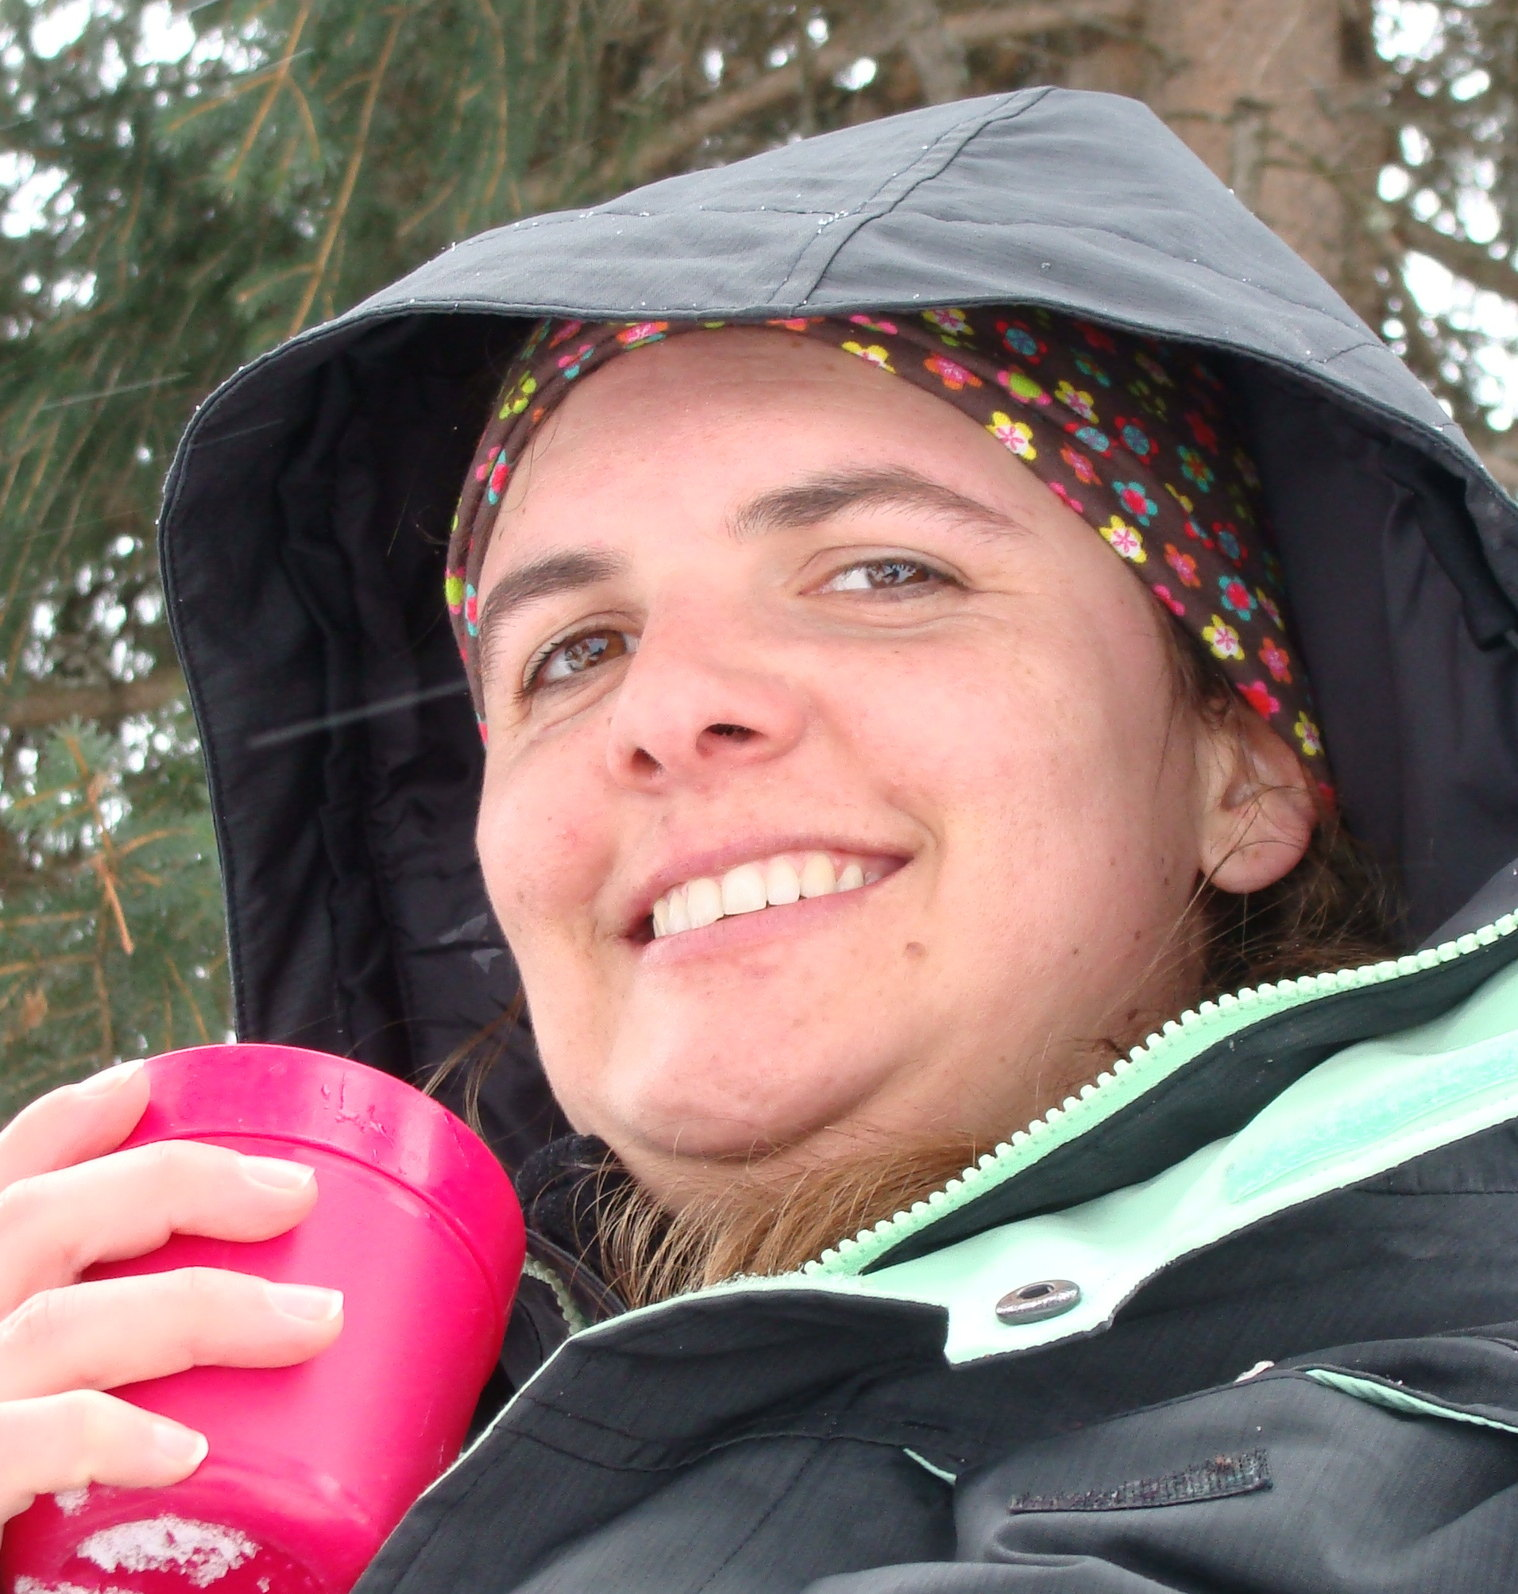
\includegraphics[width = 0.18 \textwidth]{Figures/Judith}};
				
				\node (nina) at ($(koen)+(0,-1.4)$) {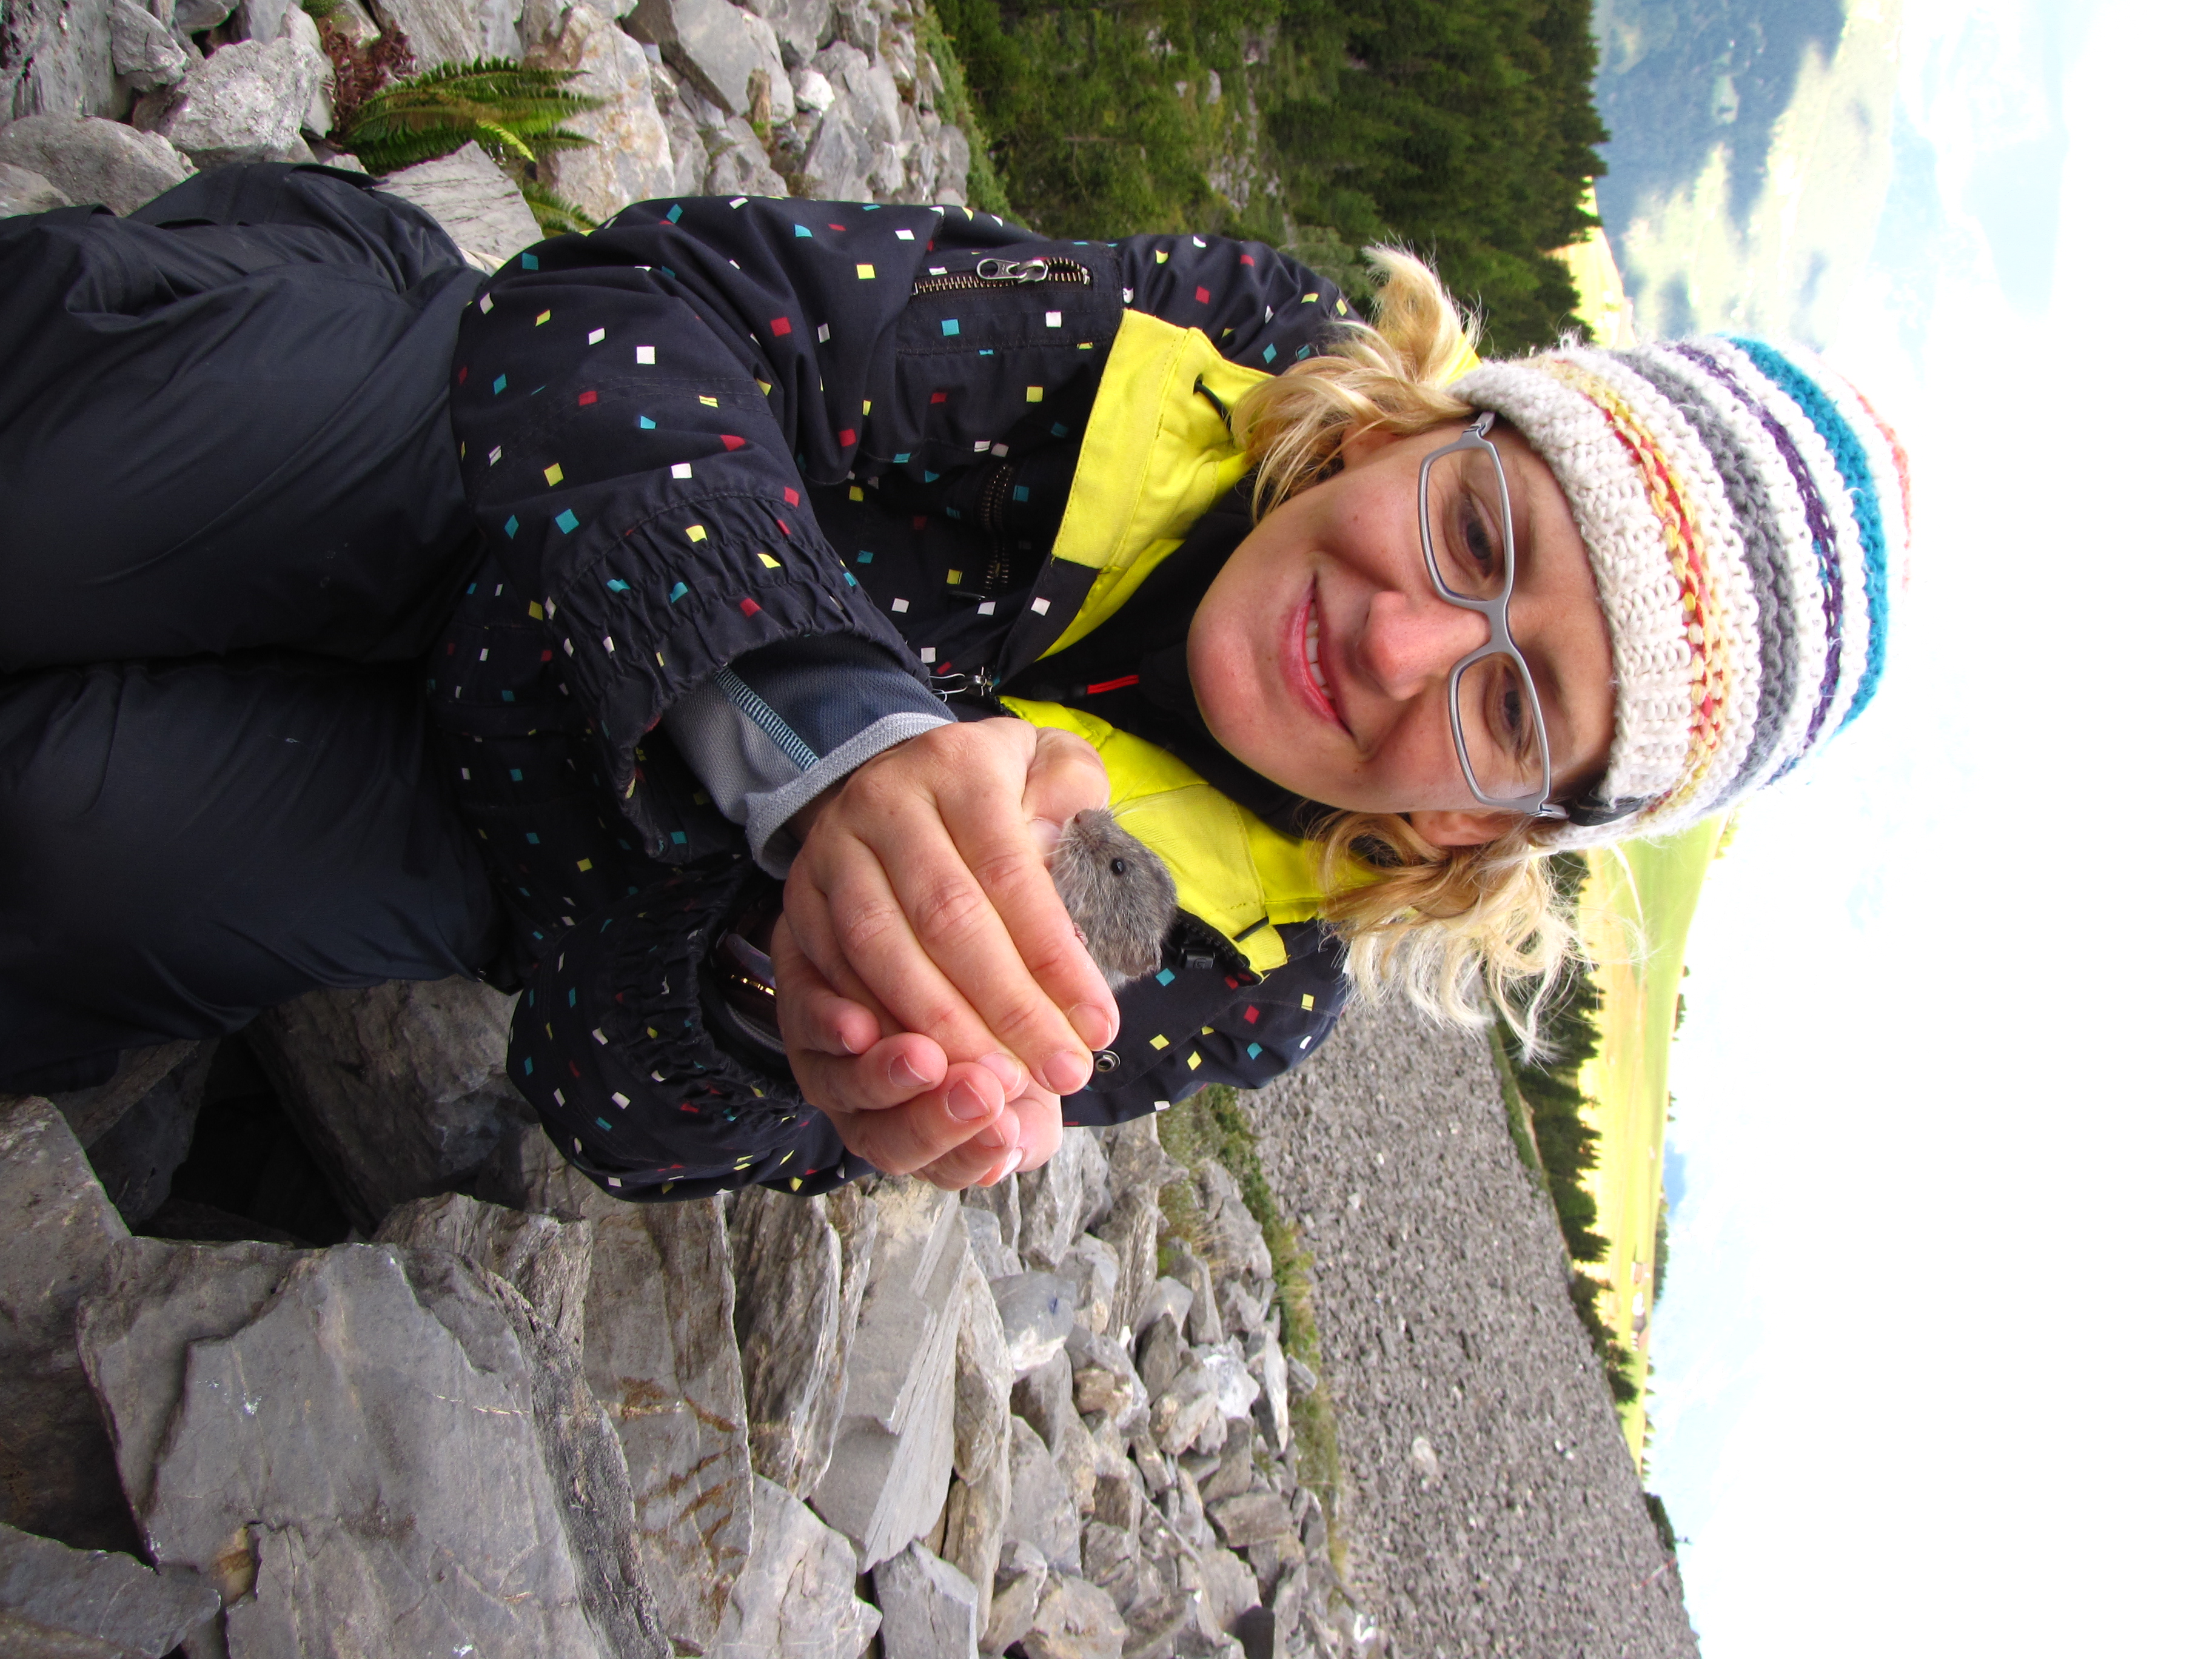
\includegraphics[width = 0.2 \textwidth]{Figures/Nina}};
				\node (hedwig) at ($(nina)+(1.2,0)$) {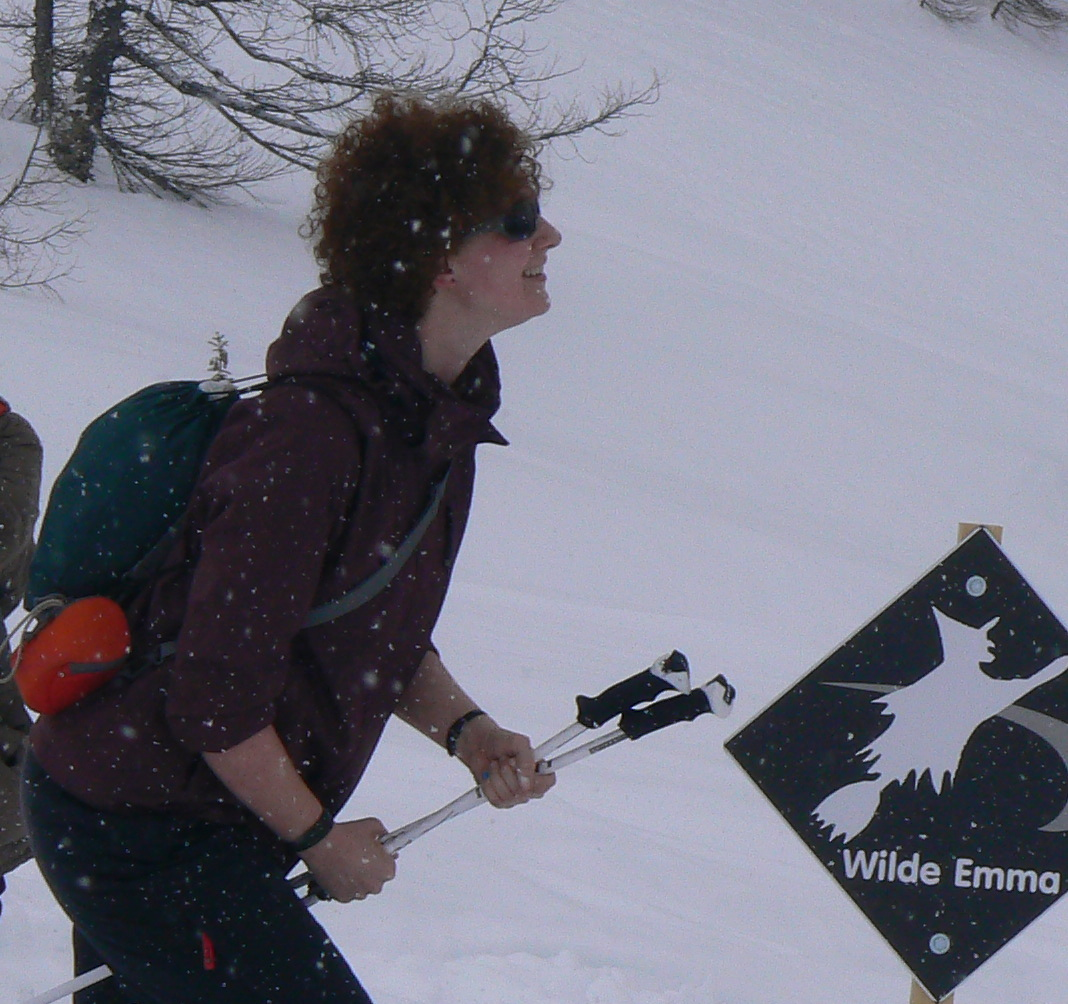
\includegraphics[width = 0.2 \textwidth]{Figures/Hedwig}};
				\node (kasia) at ($(hedwig)+(1.2,0)$) {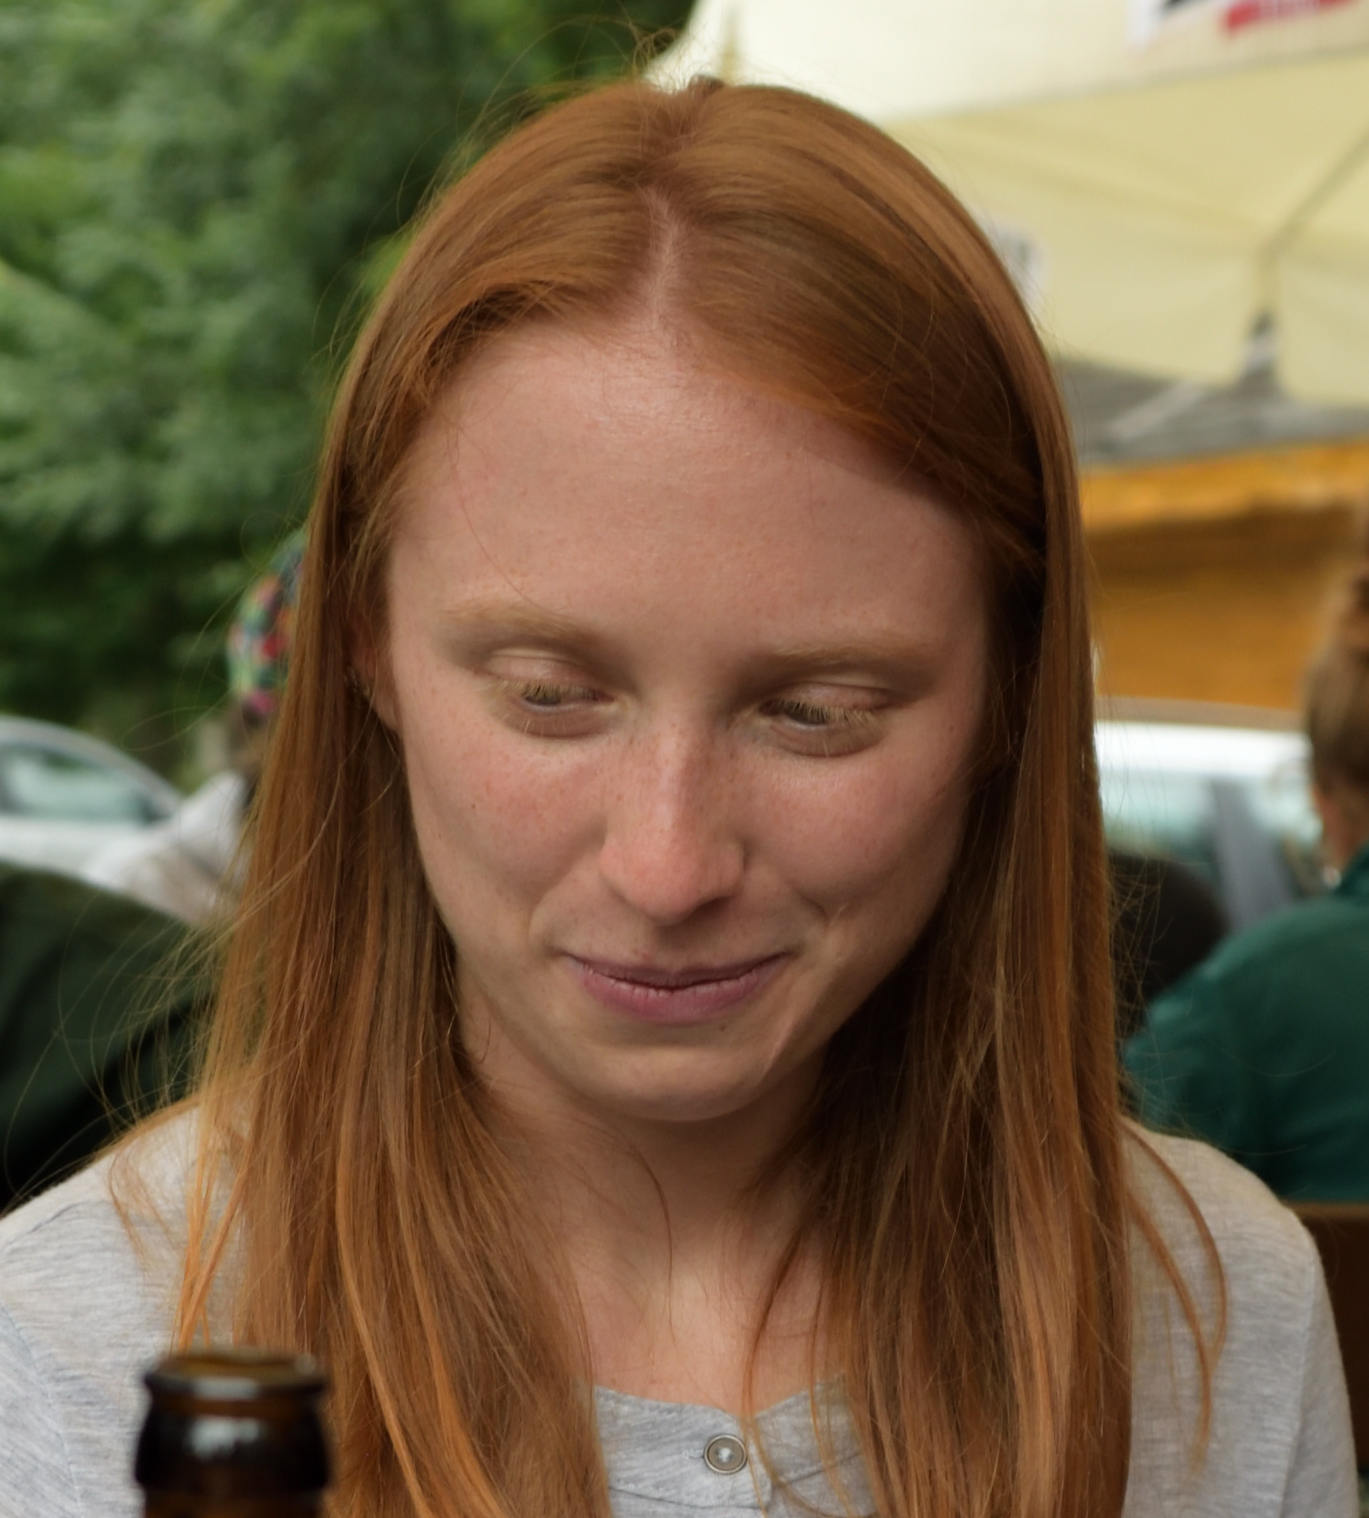
\includegraphics[width = 0.2 \textwidth]{Figures/Kasia}};
				\node (simon) at ($(kasia)+(1.2,0)$) {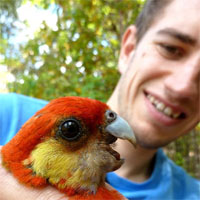
\includegraphics[width = 0.15 \textwidth]{Figures/Simon}};
				\node (chelsea) at ($(simon)+(1.3,0)$) {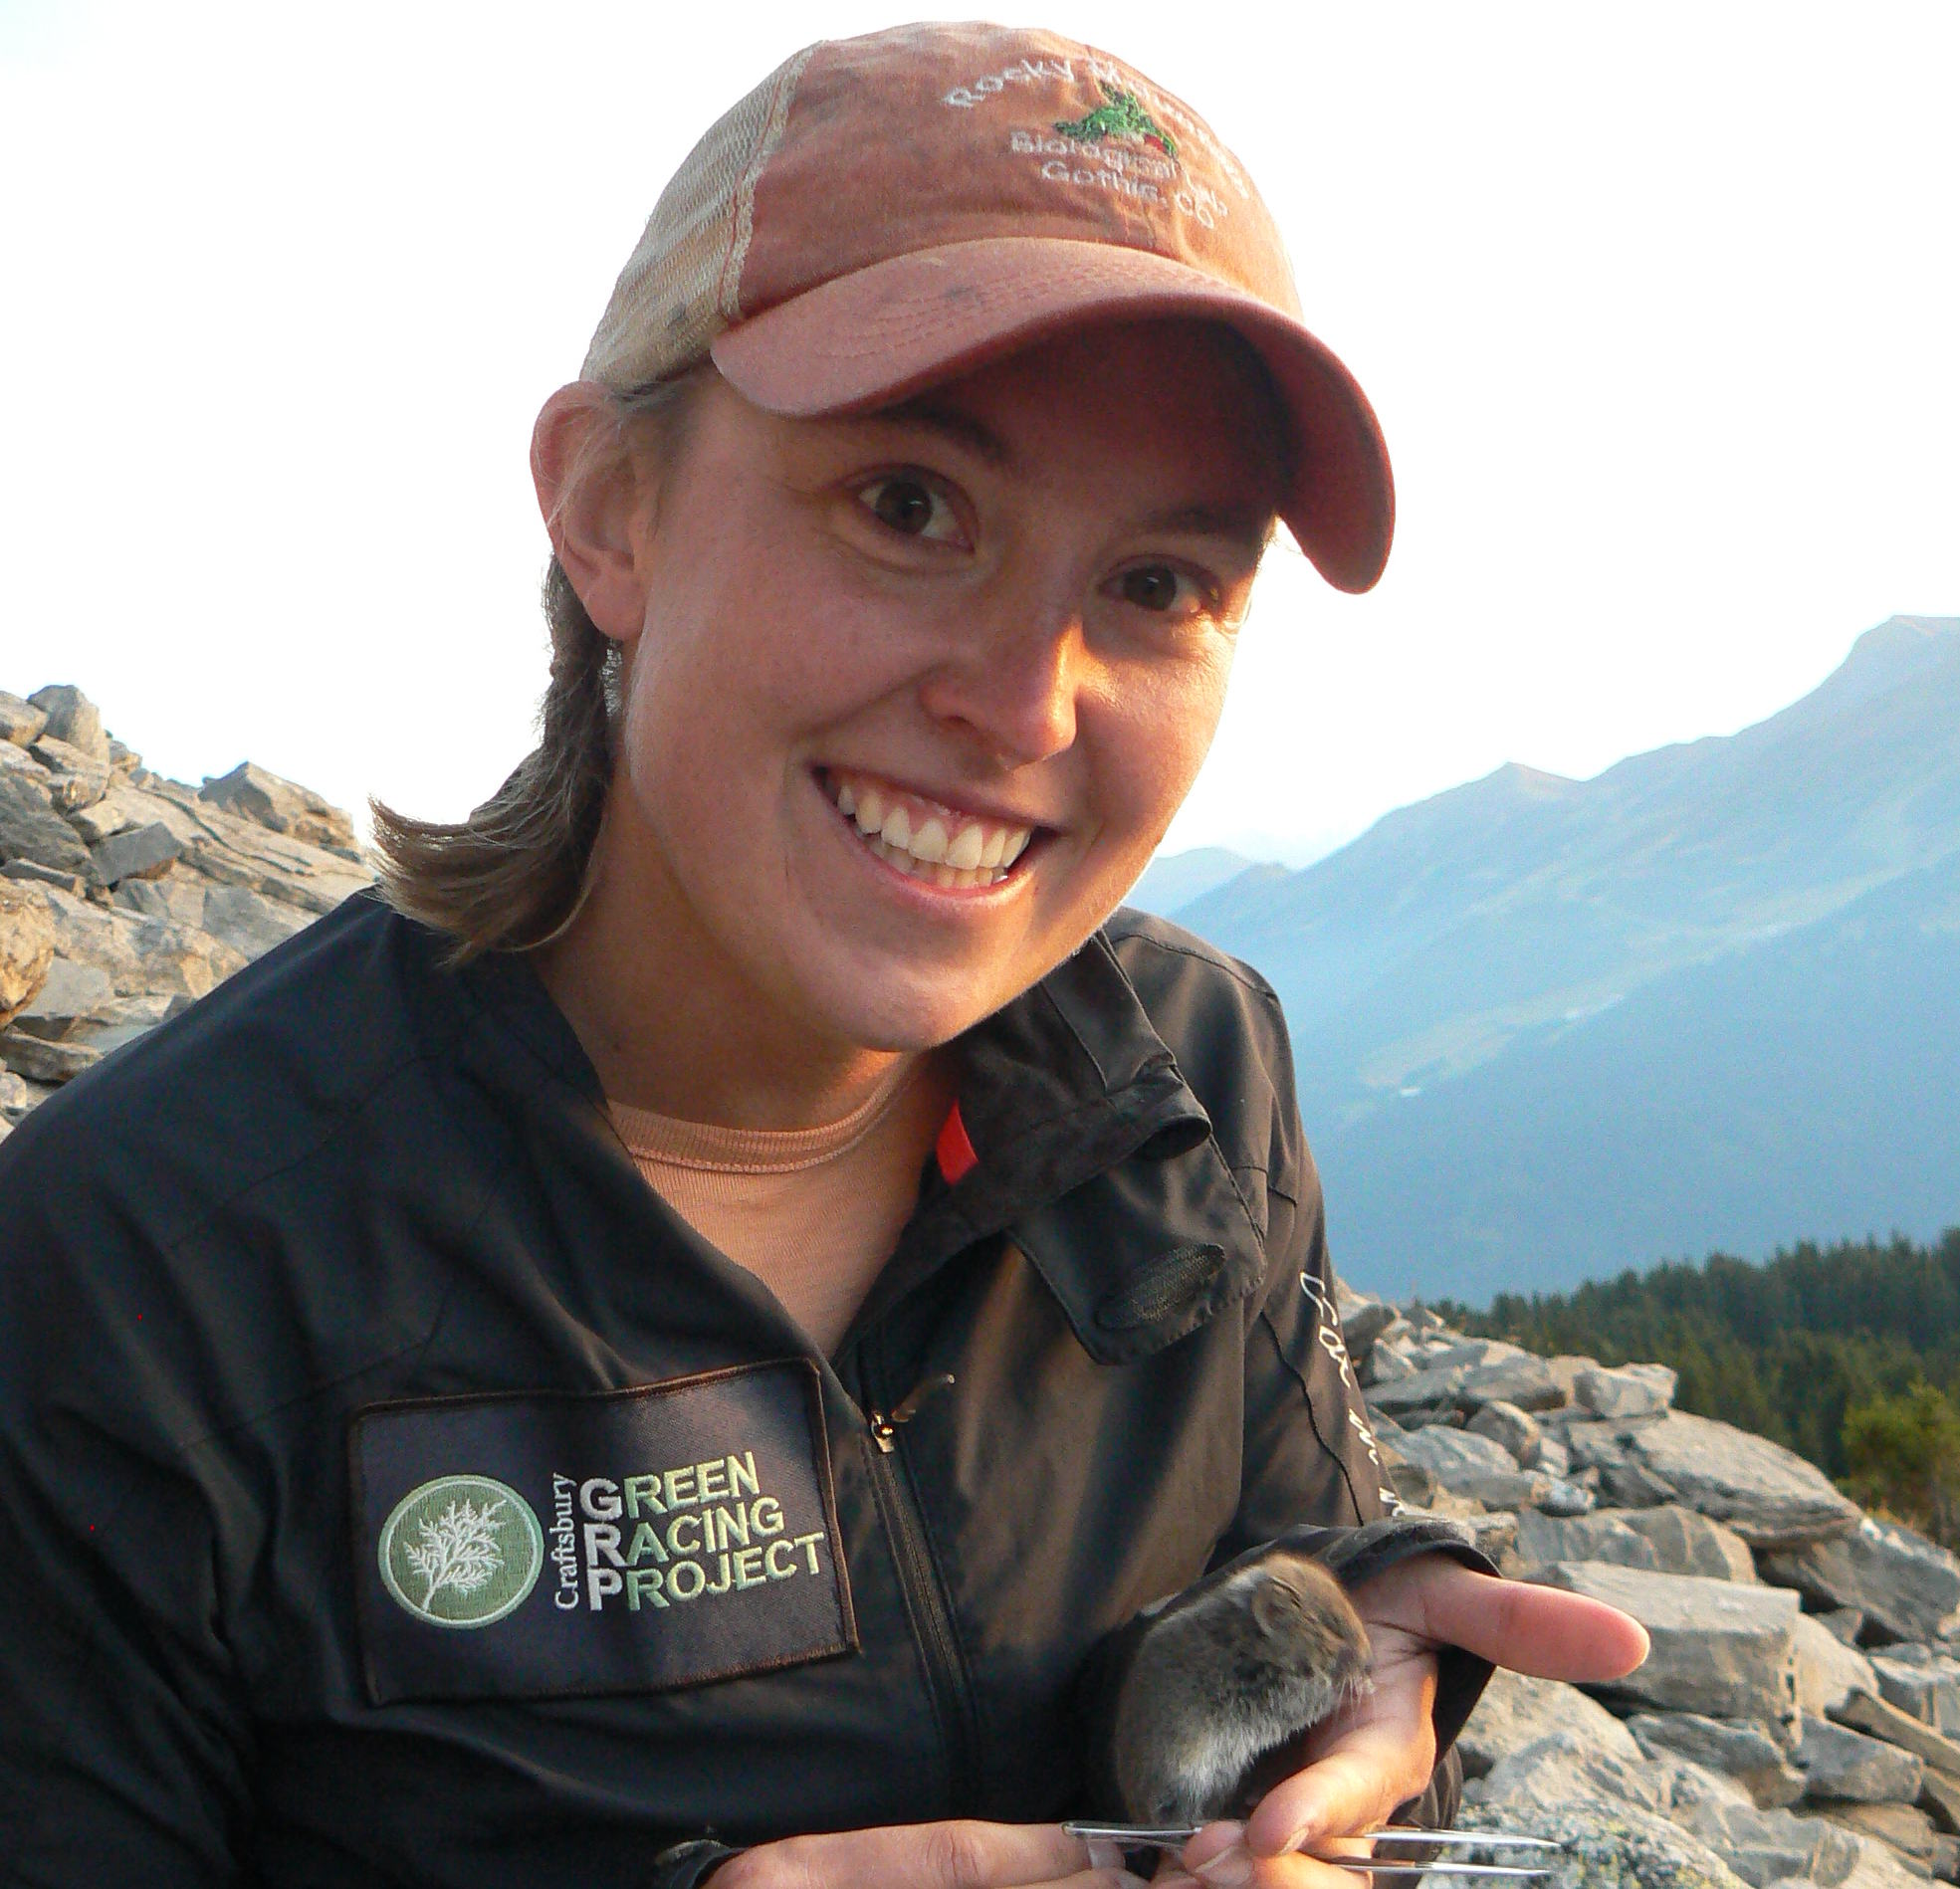
\includegraphics[width = 0.2 \textwidth]{Figures/Chelsea}};
				\node (ashley) at ($(chelsea)+(1.2,0)$) {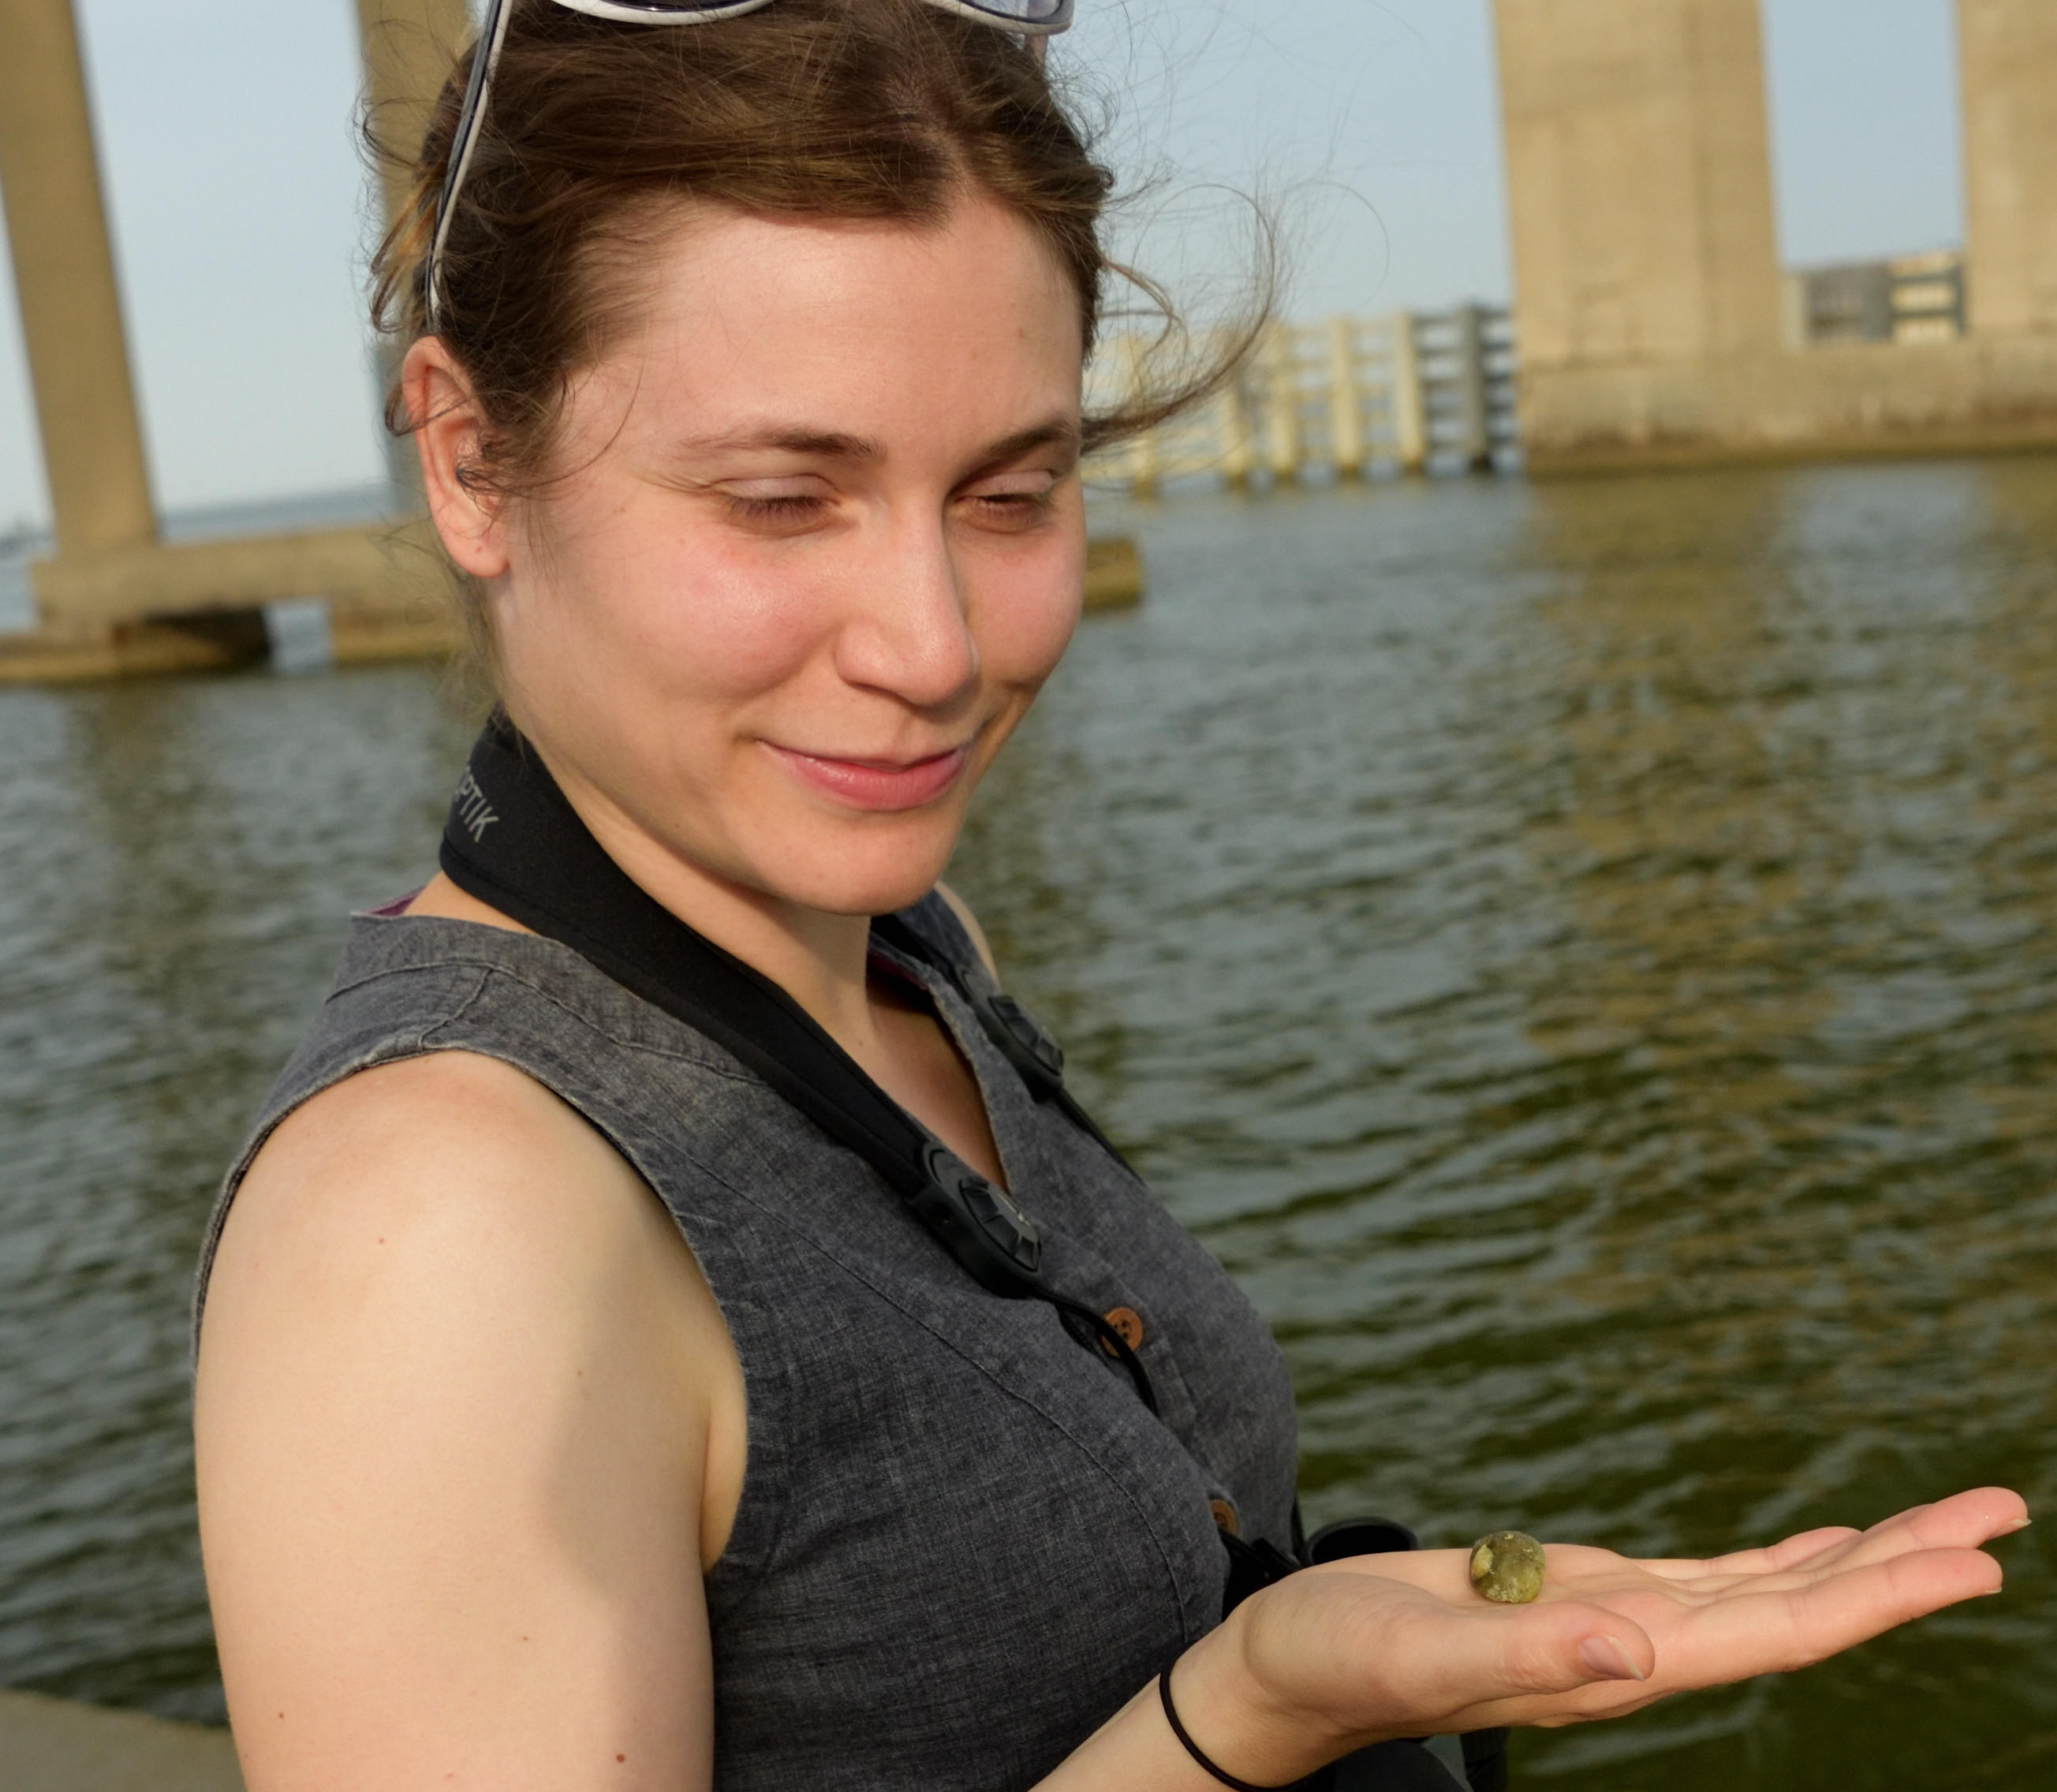
\includegraphics[width = 0.2 \textwidth]{Figures/Ashley}};

%%%%%%		
				\node (beni) at ($(nina)+(0,-1.4)$) {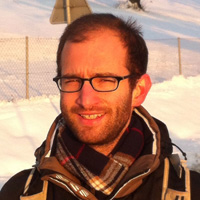
\includegraphics[width = 0.2 \textwidth]{Figures/Beni}};
				\node (alex) at ($(beni)+(1.2,0)$) {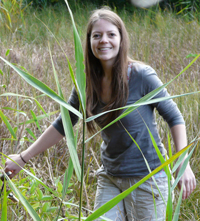
\includegraphics[width = 0.2 \textwidth]{Figures/Alex}};
				\node (rassim) at ($(alex)+(1.2,0)$) {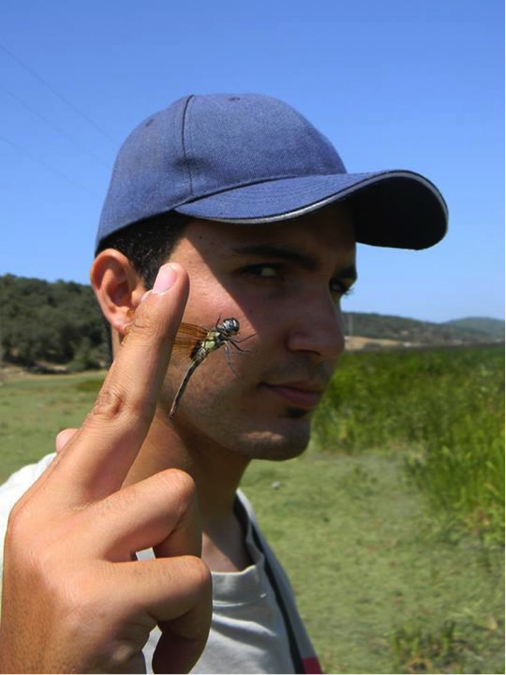
\includegraphics[width = 0.2 \textwidth]{Figures/Rassim}};
				\node (debbie) at ($(rassim)+(1.2,0)$) {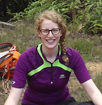
\includegraphics[width = 0.2 \textwidth]{Figures/Debbie}};
				\node (gianalberto) at ($(debbie)+(1.2,0)$) {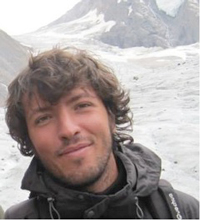
\includegraphics[width = 0.2 \textwidth]{Figures/Gianalberto}};
				\node (peter) at ($(gianalberto) +(1.2,0)$) {\includegraphics[width = 0.2 \textwidth]{Figures/Peter}};
				%%%%
				\node (jelena) at ($(beni)+(0,-1.4)$) {\includegraphics[width = 0.2 \textwidth]{Figures/Jelena}};
				\node (hanna) at ($(jelena)+(1.2,0)$) {\includegraphics[width = 0.2 \textwidth]{Figures/Hanna}};
				\node (jasmin) at ($(hanna)+(1.2,0)$) {\includegraphics[width = 0.2 \textwidth]{Figures/Jasmin}};
				\node (josh) at ($(jasmin)+(1.2,0)$)  {\includegraphics[width = 0.2 \textwidth]{Figures/Josh}};
				\node (wolf) at ($(josh)+(1.2,0)$) {\includegraphics[width = 0.2 \textwidth]{Figures/Wolf}};
				\node (bea) at ($(koen)+(0,-1.4)$) {\includegraphics[width = 0.2 \textwidth]{Figures/Bea}};
				\node (ninag) at ($(koen)+(0,-1.4)$) {\includegraphics[width = 0.2 \textwidth]{Figures/NinaG}};
				\node (anais) at ($(koen)+(0,-1.4)$) {\includegraphics[width = 0.2 \textwidth]{Figures/Anais}};
				\node (isobel) at ($(koen)+(0,-1.4)$) {\includegraphics[width = 0.2 \textwidth]{Figures/Isobel}};
				\node (erika) at ($(koen)+(0,-1.4)$) {\includegraphics[width = 0.2 \textwidth]{Figures/Erika}};
				\node (rien) at ($(koen)+(0,-1.4)$) {\includegraphics[width = 0.2 \textwidth]{Figures/Rien}};
				\node (vanja) at ($(koen)+(0,-1.4)$) {\includegraphics[width = 0.2 \textwidth]{Figures/Vanja}};
				
				\node (christine) at ($(koen)+(0,-1.4)$) {\includegraphics[width = 0.2 \textwidth]{Figures/Christine}};
				
				
			\end{tikzpicture}
		\end{figure}
	\end{column}
	\end{columns}
\end{frame}
%%%%%%%%%%%
%Intro on variation within species/population
%Explain causes of variation imply consequences

\begin{frame}{Phenotypic variation within population}
	\begin{figure}
		\includegraphics[width = 0.6 \textwidth]{Figures/Humansize}
	\end{figure}
	\begin{figure}
		\includegraphics[width = 0.45 \textwidth]{Figures/Cepaea}\hspace{0.1cm}		
		\includegraphics[width = 0.45 \textwidth]{Figures/Harmonia}
	\end{figure}
\end{frame}
%%%%%%%%%%%

\begin{frame}{Phenotypic variation within population}
	\begin{figure}
		\includegraphics[width=0.4\textwidth,height=0.3\textwidth]{Figures/babyTurtle} \hspace{1pt}
		\includegraphics[width=0.4\textwidth,height=0.3\textwidth]{Figures/adultTurtle}
		\vspace{1pt}
		\includegraphics[width=0.4\textwidth,height=0.3\textwidth]{Figures/BlueTits2}\hspace{1pt}
		\includegraphics[width=0.4\textwidth,height=0.3\textwidth]{Figures/BlueTits8}
	\end{figure}
\end{frame}
%%%%%%%%%%%

\begin{frame}{Fitness variation}
	\begin{figure}
		\includegraphics[width=0.2\textwidth,height=0.15\textwidth]{Figures/babyTurtle} \hspace{1pt}
		\includegraphics[width=0.2\textwidth,height=0.15\textwidth]{Figures/adultTurtle}
		\vspace{1pt}
		\includegraphics[width=0.2\textwidth,height=0.15\textwidth]{Figures/BlueTits2}\hspace{1pt}
		\includegraphics[width=0.2\textwidth,height=0.15\textwidth]{Figures/BlueTits8}
	\end{figure}
	
	\begin{alertblock}{What is fitness?}
		The expected relative contribution of an individual to the next generation
	\end{alertblock}
\end{frame}
%%%%%%%%%%%
%%%%%%%%%%%%%%%%%%%%%%%%%%%%%%%%%%%%%%%%%%%%%%%%%%%%%%
%%%%%%%%%%%%%%%%%%%%%%% Chap 1 %%%%%%%%%%%%%%%%%%%%%%%
%%%%%%%%%%%%%%%%%%%%%%%%%%%%%%%%%%%%%%%%%%%%%%%%%%%%%%
\section{Chance or fate? Why do survival and fertility vary?}
%Dice!
%random graph
%reality graph + examples
%two hypotheses for reality
%one dominant for a long time, challenged by new method
%
\begin{frame}

		\only<1>{
			\begin{figure}
				\includegraphics[width=\textwidth]{Figures/figure/dice1-1.pdf}
			\end{figure}}
		\only<2>{
			\begin{figure}
				\includegraphics[width=\textwidth]{Figures/figure/dice1-2.pdf}
			\end{figure}}
		\only<3>{
			\begin{figure}
				\includegraphics[width=\textwidth]{Figures/figure/dice1-3.pdf}
			\end{figure}}
		\only<4>{
			\begin{figure}
				\includegraphics[width=\textwidth]{Figures/figure/dice1-4.pdf}
			\end{figure}}
		\only<5>{
			\begin{figure}
				\includegraphics[width=\textwidth]{Figures/figure/dice1-5.pdf}
			\end{figure}}
		\only<6>{
			\begin{figure}
				\includegraphics[width=\textwidth]{Figures/figure/dice1-6.pdf}
			\end{figure}}
		\only<7>{
			\begin{figure}
				\includegraphics[width=\textwidth]{Figures/figure/dice1-7.pdf}
			\end{figure}}
	

\end{frame}
%%%%%%%%%%%

\begin{frame}

\begin{columns}
\begin{column}[c]{0.5\textwidth}
	\centering
	\textbf{One dice theory }
		\includegraphics[width=\textwidth]{Figures/figure/dice1-7.pdf}
	\end{column}
\begin{column}[c]{0.5\textwidth}
	\centering
	\uncover<2->{
	\textbf{Real pattern}
		\includegraphics[width=\textwidth]{Figures/figure/dice2-4.pdf}
	}
	
\end{column}
\end{columns}

\begin{columns}
\begin{column}[c]{0.5\textwidth}

\end{column}
\begin{column}[c]{0.5\textwidth}
\centering
	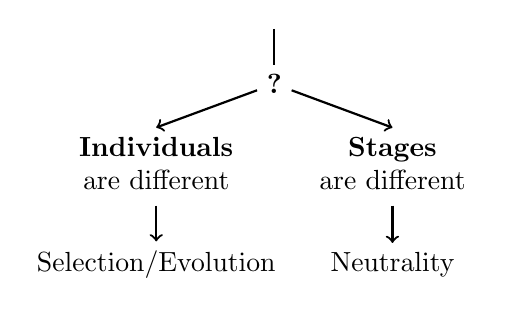
\begin{tikzpicture}
		\uncover<3->{
				\node (q) at (0,-0.7) {\textbf{?}};
				\draw[thick] (0,0) -- (q);
				\node (sel) at (-1.5,-1.5) {\parbox[t][0.2cm][t]{2cm}{\centering \textbf{Individuals} are different}};
				\draw[->, thick] (q) -- (sel.north);
		}
		\uncover<4->{	\node (neutral) at (1.5,-1.5) {\parbox[t][0.2cm][t]{1.9cm}{\centering \textbf{Stages}\\ are different}};
		\draw[->, thick] (q) -- (neutral.north);
		}
		\uncover<5->{
			\node (sh) at (-1.5, -3) {Selection/Evolution};
			\node (ne) at (1.5, -3)  {Neutrality};
			\draw[->, thick] ($(sel.south)+(0,-0.5)$) -- (sh.north);
			\draw[->, thick] ($(neutral.south)+(0,-0.5)$) -- (ne.north);
		}
	
	\end{tikzpicture}
\end{column}
\end{columns}

\end{frame}
%%%%%%%%%%%

\begin{frame}{The neutral theory}
\includegraphics[width=\textwidth]{Figures/NeutralTheory}

\textbf{Neutral matrix method}
\vspace{0.5cm}
\begin{columns}
\begin{column}[c]{0.5\textwidth}
\begin{table}
\begin{tabular}{c|c c c}
& \multicolumn{3}{c}{next year} \\
	& 1 & 2 & 3\\
	\hline
1	& \color{red!90}{0.9}	&	 \color{red!8}{0.08}	&	 \color{red!2}{0.02}	\\
2 & 0  	&	\color{red!70}{0.7}	&	 \color{red!30}{0.3}	\\
3 & 0  	&	 \color{red!20}{0.2}	&	\color{red!80}{0.8}	\\

\end{tabular}
\end{table}
\end{column}
\begin{column}[c]{0.5\textwidth}
	\only<3>{
	\vspace{-1cm}
		\begin{figure}
		\includegraphics[width=1\textwidth]{Figures/figure/lrssimul-1.pdf}
		\end{figure}}
	\only<4>{
	\vspace{-1cm}
	\begin{figure}
	\includegraphics[width=1\textwidth]{Figures/figure/lrssimul-3.pdf}
	\end{figure}}
\end{column}
\end{columns}
\centering
\textbf{\color{OwlRed}{No variation in fitness among individuals}}
\end{frame}
%%%%%%%%%%%
\begin{frame}{Conflicting results}
\begin{columns}
	\begin{column}[c]{0.5\textwidth}
	\textbf{\color{OwlRed}{Neutral matrix method}}
	\begin{itemize}
		\uncover<2->{\item No significant differences between individuals}
		\uncover<4->{\item \dots because of stage structure}
		\uncover<6->{\item \dots very little and due to chance only}
	\end{itemize}
	
	\end{column}
	\begin{column}[c]{0.5\textwidth}
	\textbf{\color{OwlBlue}{Mixed model method \& Quantitative genetics}}

	\begin{itemize}
		\uncover<3->{\item Individual performances are repeatable}
		\uncover<5->{\item \dots fitness traits are heritable} 
		\uncover<7->{\item \dots eh?}
	\end{itemize}
	
	\end{column}
\end{columns}

\begin{figure}
	\only<1>{\includegraphics[width=0.4\textwidth]{Figures/Kittiwake}}
	\only<2>{\includegraphics[width=0.8\textwidth]{Figures/Steinerkittiwake}}
	\only<3>{\vspace{-2cm} \includegraphics[width=0.8\textwidth]{Figures/CamKittiwake}}
	\only<4>{\vspace{-1.5cm}\includegraphics[width=0.8\textwidth]{Figures/figure/dice2-4.pdf}\vspace{-1.5cm}}
\end{figure}

\only<8>{\begin{block}{Why?}
	\begin{itemize}
		\item \textbf{\color{OwlRed}{Neutral matrix method}} =\textbf{false negative}?
		\item \textbf{\color{OwlBlue}{Mixed model method}} =\textbf{false positive}?
	\end{itemize}
\end{block}}

\end{frame}
%%%%%%%%%%%

\begin{frame}{Method}
\begin{figure}
\begin{tikzpicture}[%
  % common options for blocks:
  block/.style = {draw, align=center, anchor=north,
              minimum height=0.50cm, inner sep=1pt,fill=black!80},
	roundblock/.style = {draw, align=center, anchor=north,
              minimum height=2cm, inner sep=2pt,rounded corners=3pt,fill=black!80},
	backblock/.style = {fill=gray!90, align=center, anchor=west,
               inner sep=2pt,rounded corners=3pt},
  % common options for the circles:
  ball/.style = {circle, draw, align=center, anchor=north, inner sep=0},
	oval/.style = {ellipse, draw, align=center, anchor=north, inner sep=1pt,fill=white}
	]
\footnotesize	
\node[backblock,minimum width=5.25cm,minimum height=5.2cm] (Abb) at (-4,-1) {};
\node[backblock,fill=gray!75,minimum width=5.25cm,minimum height=5.2cm] (Bbb) at ($(Abb.east) +(0.25,0)$) {};
\node[] (a) at ($(Abb.north)+(-1,-0.25)$){\textbf{Simulate data}};
\node[] (b) at ($(Bbb.north)+(-0.5,-0.25)$) {\textbf{Test fixed heterogeneity}};

\node[roundblock,text width=2cm, anchor=west] (Parameters) at ($(Abb.west)+(0.25,0)$) {\textbf{Parameters}\\ Fertility, Viability, Persistence, \textbf{\color{OwlYellow}{Individual differences}}};

{\scriptsize 
\node[block,text width=1.5cm] (scenario1) at ($(Parameters.north)+(2.2,0)$) {Scenario 1};
\node[text width=2cm, align=center] (par) at ($(scenario1)+(0,0.8)$) {Parameter};
\node[text width=2cm, align=center] (comb) at ($(par)+(0,-0.3)$) {combinations};
\node[block,text width=1.5cm] (scenario2) at ($(scenario1)+(0,-0.6)$) {Scenario 2};
\node[] (scenarion) at ($(scenario1)+(0,-1.45)$) {\textbf{\vdots}};
\node[block,text width=1.5cm] (scenario240) at ($(scenario1)+(0,-2)$) {Scenario 249};
}

\draw[->,shorten >= 2pt] (Parameters.east) to (scenario1.west);
\draw[->,shorten >= 2pt] (Parameters.east) to (scenario2.west);
\draw[->,shorten >= 2pt] (Parameters.east) to (scenario240.west);


{\scriptsize 
\coordinate (stos) at (1.8,0);
\node[backblock,text width=1.8cm, anchor=west, fill=black!80] (simdata1) at ($(scenario1.west) + (stos)$) {1000 data sets};
\node[backblock,text width=1.8cm, anchor=west, fill=black!80] (simdata2) at ($(scenario2.west) + (stos)$) {1000 data sets};
\node[] (simn) at ($(scenarion)+(stos)$) {\textbf{\vdots}};
\node[backblock,text width=1.8cm, anchor=west, fill=black!80] (simdata240) at ($(scenario240.west) + (stos)$) {1000 data sets};
}

\draw[->] (scenario1.east) to (simdata1.west);
\draw[->] (scenario2.east) to (simdata2.west);
\draw[->] (scenario240.east) to (simdata240.west);

{\scriptsize 
\gettikzxy{(simdata1.east)}{\ax}{\ay}
\gettikzxy{(Parameters.north)}{\px}{\py}
\coordinate (cordtest) at ($(\ax,\py)+(2.5,0)$);
\node[roundblock,text width=3cm,minimum height=0.2cm] (test) at (cordtest) {\tikz{\node[anchor=north] (ts) at (0.125,0.6) {\centering\textbf{\color{OwlYellow}{Individual differences?}}};
\node[roundblock,text width=2.6cm,minimum height=0.2cm] (MM) at (0,-0.1) {\parbox[t][0.2cm][t]{2.6cm}{\centering\textbf{\color{OwlBlue}{Mixed models}}}};
\node[roundblock,text width=2.6cm,minimum height=0.2cm] (MM) at (0,-0.6) {\parbox[t][0.2cm][t]{2.6cm}{\centering\textbf{\color{OwlRed}{Neutral matrices}}}};
}};
}

\draw[->,shorten >= 2pt] (simdata1.east) to (test.170);
\draw[->,shorten >= 2pt] (simdata2.east) to (test.180);
\draw[->,shorten >= 2pt] (simdata240.east) to (test.190);

\node[block, anchor=south] (error) at ($(Bbb.south)+(0,0.25)$) {False positive and false negative rates};

\draw[->, shorten >= 2pt] (test.270) to (error.90);

\end{tikzpicture}
\end{figure}
\end{frame}
%%%%%%%%%%%

\begin{frame}{Results}
\only<1>{
\begin{figure}
	\includegraphics[width=\textwidth]{Figures/figure/resultsdynhet-2.pdf}
\end{figure}}
\only<2>{
\begin{figure}
	\includegraphics[width=\textwidth]{Figures/figure/resultsdynhet-3.pdf}
\end{figure}}
\only<3>{
\begin{figure}
	\includegraphics[width=\textwidth]{Figures/figure/resultsdynhet-4.pdf}
\end{figure}}
	
\end{frame}
%%%%%%%%%%%
\begin{frame}{Conclusion}

\begin{block}{Why conflicting methods?}
	\uncover<2->{\begin{itemize}
		\item \textbf{\color{OwlRed}{Neutral matrix method}} =\textbf{false negative}? \textbf{\color{red}{YES}}
		\item \textbf{\color{OwlBlue}{Mixed model method}} =\textbf{false positive}? \textbf{\color{red}{NO}}
	\end{itemize}}
	\uncover<3->{$\rightarrow$ Individual differences in fitness components are common}
\end{block}

	\uncover<4->{\begin{block}{Implications}
		\begin{itemize}
			\uncover<5->{\item Phenotypic variation in fitness $\rightarrow$ opportunity for selection}
			\uncover<6->{\item Heritability of fitness $=$ \textbf{evolution}}
		\end{itemize}
	\end{block}}
	
	\uncover<6->{
	\begin{figure}
		\begin{tikzpicture}
			\node (f) at (-1,0) {\includegraphics[width = 0.2\textwidth]{Figures/Fisher}};
			\node (fn) at ($(f.south)+(0,-0.2)$) {\textbf{R.A. Fisher}};
			\node (p) at (1,0) {\includegraphics[width = 0.2\textwidth]{Figures/Price}};
			\node (fn) at ($(p.south)+(0,-0.2)$) {\textbf{G. Price}};
		\end{tikzpicture}
	\end{figure}}
\end{frame}
%%%%%%%%%%%
\begin{frame}
\end{frame}
%%%%%%%%%%%
%%%%%%%%%%%%%%%%%%%%%%%%%%%%%%%%%%%%%%%%%%%%%%%%%%%%%%
%%%%%%%%%%%%%%%%%%%%%%% Chap 2 %%%%%%%%%%%%%%%%%%%%%%%
%%%%%%%%%%%%%%%%%%%%%%%%%%%%%%%%%%%%%%%%%%%%%%%%%%%%%%

\begin{frame}{Evolution in a changing world}

	\only<1>{\begin{figure}
		\includegraphics[width = 0.6\textwidth]{Figures/ipcc}
		
		Intergovernmental panel on climate change 5th Report (2014)
	\end{figure}}
	
	\only<2>{\begin{figure}
		\includegraphics[width = 0.8\textwidth]{Figures/biodiv}
		
		Newbold \& al. (2016). Has land use pushed terrestrial biodiversity beyond the planetary boundary? A global assessment. Science, 353
	\end{figure}}
	
	\only<3>{\begin{figure}
		\includegraphics[width = 0.8\textwidth]{Figures/parmesan}
		\end{figure}}
	
\end{frame}
%%%%%%%%%%%

\begin{frame}

	\begin{figure}
		\begin{tikzpicture}
			\uncover<1-2>{\node [shading = axis,rectangle, bottom color=green!50!gray, top color=gray, minimum height=2.5cm, minimum width=5.5cm] (hab1) at (0,0) {};}
			
			\uncover<3->{\node [shading = axis,rectangle, bottom color=green, top color=green!50!gray, minimum height=2.5cm, minimum width=5.5cm] (hab1) at (0,0) {};}
			
			\uncover<1>{\node (sun) at ($(hab1.150)+(-1,1)$) {\includegraphics[width = 0.10\textwidth]{Figures/sun.png}};}
			\uncover<2->{\node (sun) at ($(hab1.150)+(-1,1)$) {\includegraphics[width = 0.15\textwidth]{Figures/sun.png}};}
			
			\uncover<1-3>{\node (vole1) at (0,0) {\includegraphics[width = 0.05\textwidth]{Figures/snowwwvole2}};
			\node (vole2) at (1,0.1) {\includegraphics[width = 0.06\textwidth]{Figures/snowwwvole2}};
			\node (vole3) at (-0.7,0.3) {\includegraphics[width = 0.03\textwidth]{Figures/snowwwvole2}};
			\node (vole4) at (-1.5,-0.3) {\includegraphics[width = 0.06\textwidth]{Figures/snowwwvole2}};
			\node (vole5) at (1.7,-0.15) {\includegraphics[width = 0.04\textwidth]{Figures/snowwwvole2}};}
			
			\uncover<4>{
			\node [shading = axis,rectangle, bottom color=green, top color=green!50!gray, minimum height=2.5cm, minimum width=5.5cm] (hab2) at ($(hab1)+(0,0)$) {};
			\node (vole1b) at (0,2) {\includegraphics[width = 0.05\textwidth]{Figures/snowwwvole2}};
			\node (vole2b) at (1,2.3) {\includegraphics[width = 0.06\textwidth]{Figures/snowwwvole2}};
			\node (vole3b) at (-0.7,2.3) {\includegraphics[width = 0.03\textwidth]{Figures/snowwwvole2}};
			\node (vole4b) at (-1.5,1.7) {\includegraphics[width = 0.06\textwidth]{Figures/snowwwvole2}};
			\node (vole5b) at (1.7,1.25) {\includegraphics[width = 0.04\textwidth]{Figures/snowwwvole2}};}	
			
			\uncover<5>{\node (vole1c) at (0,0) {\includegraphics[width = 0.08\textwidth]{Figures/Deadsnowwwvole2}};
			\node (vole2c) at (1,0.1) {\includegraphics[width = 0.09\textwidth]{Figures/Deadsnowwwvole2}};
			\node (vole3c) at (-0.7,0.3) {\includegraphics[width = 0.05\textwidth]{Figures/Deadsnowwwvole2}};
			\node (vole4c) at (-1.5,-0.3) {\includegraphics[width = 0.09\textwidth]{Figures/Deadsnowwwvole2}};
			\node (vole5c) at (1.7,-0.15) {\includegraphics[width = 0.06\textwidth]{Figures/Deadsnowwwvole2}};}

			\uncover<6>{\node (vole1q) at (0,0) {\includegraphics[width = 0.05\textwidth]{Figures/snowwwvole2}};
			\node (vole2q) at (1,0.1) {\includegraphics[width = 0.06\textwidth]{Figures/snowwwvole2}};
			\node (vole3q) at (-0.7,0.3) {\includegraphics[width = 0.03\textwidth]{Figures/snowwwvole2}};
			\node (vole4q) at (-1.5,-0.3) {\includegraphics[width = 0.06\textwidth]{Figures/snowwwvole2}};
			\node (vole5q) at (1.7,-0.15) {\includegraphics[width = 0.04\textwidth]{Figures/snowwwvole2}};}
			
			\uncover<7>{\node (vole1s) at (0,0) {\includegraphics[width = 0.06\textwidth]{Figures/snowwwvole2}};
			\node (vole2s) at (1,0.1) {\includegraphics[width = 0.07\textwidth]{Figures/snowwwvole2}};
			\node (vole3s) at (-0.7,0.3) {\includegraphics[width = 0.04\textwidth]{Figures/snowwwvole2}};
			\node (vole4s) at (-1.5,-0.3) {\includegraphics[width = 0.07\textwidth]{Figures/snowwwvole2}};
			\node (vole5s) at (1.7,-0.15) {\includegraphics[width = 0.05\textwidth]{Figures/snowwwvole2}};}
			
						\uncover<8>{\node (vole1x) at (0,0) {\includegraphics[width = 0.05\textwidth]{Figures/snowwwvole2}};
			\node (vole2x) at (1,0.1) {\includegraphics[width = 0.06\textwidth]{Figures/snowwwvole2}};
			\node (vole3x) at (-0.7,0.3) {\includegraphics[width = 0.03\textwidth]{Figures/snowwwvole2}};
			\node (vole4x) at (-1.5,-0.3) {\includegraphics[width = 0.06\textwidth]{Figures/snowwwvole2}};
			\node (vole5x) at (1.7,-0.15) {\includegraphics[width = 0.04\textwidth]{Figures/snowwwvole2}};}
			
			\uncover<9>{\node (vole1e) at (0,0) {\includegraphics[width = 0.08\textwidth]{Figures/Deadsnowwwvole2}};
			\node (vole2e) at (1,0.3) {\includegraphics[width = 0.06\textwidth]{Figures/snowwwvole2}};
			\node (vole3e) at (-0.7,0.3) {\includegraphics[width = 0.05\textwidth]{Figures/Deadsnowwwvole2}};
			\node (vole4e) at (-1.5,-0.3) {\includegraphics[width = 0.06\textwidth]{Figures/snowwwvole2}};
			\node (vole5e) at (1.7,-0.15) {\includegraphics[width = 0.06\textwidth]{Figures/Deadsnowwwvole2}};}
			
			\uncover<10>{\node (vole1f) at (0,0) {\includegraphics[width = 0.065\textwidth]{Figures/snowwwvole2}};
			\node (vole2f) at (1,0.3) {\includegraphics[width = 0.06\textwidth]{Figures/snowwwvole2}};
			\node (vole3f) at (-0.7,0.3) {\includegraphics[width = 0.075\textwidth]{Figures/snowwwvole2}};
			\node (vole4f) at (-1.5,-0.3) {\includegraphics[width = 0.062\textwidth]{Figures/snowwwvole2}};
			\node (vole5f) at (1.7,-0.15) {\includegraphics[width = 0.058\textwidth]{Figures/snowwwvole2}};}
			
		\end{tikzpicture}
	\end{figure}

\end{frame}
%%%%%%%%%%%



\section{Evolution or plasticity? What drives phenotypic change?}

\begin{frame}

\end{frame}


%%%%%%%%%%%%%%%%%%%%%%%%%%%%%%%%%%%%%%%%%%%%%%%%%%%%%%%%%%%%%%%%%%%%%%%
%%%%%%%%%%%%%%%%%%%%%%%%%%%% Monitoring %%%%%%%%%%%%%%%%%%%%%%%%%%%%%%%
%%%%%%%%%%%%%%%%%%%%%%%%%%%%%%%%%%%%%%%%%%%%%%%%%%%%%%%%%%%%%%%%%%%%%%%

%FIeld and population
\begin{frame}[plain]{}
	\begin{figure}
	\centering
		\includegraphics[height= \textheight]{Figures/SnowBall}
	\end{figure}
\end{frame}
%%%%%%%%%%%

\begin{frame}{Snow vole (\textit{Chionomys nivalis}, Martins 1842)}

\begin{columns}
	\begin{column}[c]{0.5\textwidth}
		\begin{itemize}[<+->]
			\item NOT white
			\item Rock-dweller
			\item 30-45g
			\item 10-14cm long $+$ 5-8cm tail
			\item Slow life pace
		\end{itemize}
	\end{column}
	\begin{column}[c]{0.5\textwidth}
	\begin{figure}
	\centering
		\includegraphics[width= \textwidth]{Figures/P1250035}
	\end{figure}
	\end{column}
	\end{columns}
\end{frame}
%%%%%%%%%%%

\begin{frame}[plain]{}
	\begin{figure}
	\centering
		\includegraphics[height= \textheight]{Figures/map-1}
	\end{figure}
\end{frame}
%%%%%%%%%%%

\begin{frame}[plain]{}
	\begin{figure}
	\centering
		\begin{tikzpicture}
			
			\node (pic) at (0,0) {\includegraphics[width= 0.95\textwidth]{Figures/DSC_2111viewontaliflue}};
			\draw[rounded corners,thick,color=red] (-1.2,-0.8) rectangle (0.5,0);
		\end{tikzpicture}
	\end{figure}
\end{frame}
%%%%%%%%%%%

\begin{frame}[plain]{}
	\begin{figure}
	\centering
		\includegraphics[width= \textwidth]{Figures/fieldposts2}
	\end{figure}
\end{frame}
%%%%%%%%%%%

\begin{frame}[plain]{}
	\begin{figure}
	\centering
		\includegraphics[width= \textwidth]{Figures/boulder}
	\end{figure}
\end{frame}
%%%%%%%%%%%

\begin{frame}[plain]{}
	\begin{figure}
	\centering
		\includegraphics[width= \textwidth]{Figures/DSC_2027trap}
	\end{figure}
\end{frame}
%%%%%%%%%%%

\begin{frame}{What we measure}

\begin{columns}
	\begin{column}[c]{0.4\textwidth}
		\begin{itemize}
			\item<2-> Morphology
				\begin{itemize}
					\item Body mass 
					\item Body length
					\item Tail length
				\end{itemize}
			\item<3-> Capture/Recaptures
				\begin{itemize}
					\item Death/emigration
					\item Location
				\end{itemize}
			\item<4-> DNA
				\begin{itemize}
					\item 20 ``neutral'' markers
					\item Sex identification
					\item Any genotyping
					\item<5-> \textbf{Pedigree}
				\end{itemize}
		\end{itemize}
	\end{column}
	
	\begin{column}[c]{0.6\textwidth}

	\centering
		\only<2>{\includegraphics[height= \textheight]{Figures/CN2015_MeulenbroekLiz_00024}}
		\only<3>{\includegraphics[height= \textheight]{Figures/CN2015_MeulenbroekLiz_00022}}
		\only<4>{\includegraphics[height= \textheight]{Figures/IMG_20160916_075241}}
		\only<5>{\includegraphics[height= 0.5\textheight]{Figures/familytree}}
		\only<6>{\includegraphics[height= \textheight]{Figures/pedigreeplot}}

	\end{column}
\end{columns}
\end{frame}
%%%%%%%%%%%


%%%%%%%%%%%%%%%%%%%%%%%%%%%%%%%%%%%%%%%%%%%%%%%%%%%%%%
%%%%%%%%%%%%%%%%%%%%%%% Chap 3 %%%%%%%%%%%%%%%%%%%%%%%
%%%%%%%%%%%%%%%%%%%%%%%%%%%%%%%%%%%%%%%%%%%%%%%%%%%%%%
\section{Are snow vole evolving? Why?}

%Open some dice! -> DNA and grass in it, leading to most common number...

%%%%%%%%%%%%%%%%%%%%%%%%%%%%%%%%%%%%%%%%%%%%%%%%%%%%%%
%%%%%%%%%%%%%%%%%%%%%%% Chap 4 %%%%%%%%%%%%%%%%%%%%%%%
%%%%%%%%%%%%%%%%%%%%%%%%%%%%%%%%%%%%%%%%%%%%%%%%%%%%%%

\section{Do selection and evolution fluctuate?}

%%%%%%%%%%%%%%%%%%%%%%%%%%%%%%%%%%%%%%%%%%%%%%%%%%%%%%
%%%%%%%%%%%%%%%%%%%%%%% Conclu %%%%%%%%%%%%%%%%%%%%%%%
%%%%%%%%%%%%%%%%%%%%%%%%%%%%%%%%%%%%%%%%%%%%%%%%%%%%%%

\section{What is left?}

\end{document}
